
\chapter{Clustering Experiments}
\label{ch:Clustering Experiments}
\thispagestyle{myheadings}

\section{Experiments Setup}

In the experiments, six sets of admixtures are tested with many different clusterers. The six sets of admixtures are combinations of EPG sample types and whether high-pass filtering of EPGs is used. They are listed in Table \ref{table:Sets of simulated admixtures}.

In each set, there are the 11 admixture types described in Table \ref{table:Admixture types simulated}. Each admixture type consists of 1,000 trial runs of simulated admixtures that are generated by pseudo-random sampling of the available EPGs.

\begin{table}
\centering
\begin{tabular}{lll}
\toprule
                                   Name & Sample Type & High-pass Filtering \\
\midrule
 highpass\_0-sampleids\_saliva-nruns\_1000 & Saliva only &                  No \\
highpass\_71-sampleids\_saliva-nruns\_1000 & Saliva only &                 Yes \\
  highpass\_0-sampleids\_blood-nruns\_1000 &  Blood only &                  No \\
 highpass\_71-sampleids\_blood-nruns\_1000 &  Blood only &                 Yes \\
    highpass\_0-sampleids\_all-nruns\_1000 &         All &                  No \\
   highpass\_71-sampleids\_all-nruns\_1000 &         All &                 Yes \\
\bottomrule
\end{tabular}
\caption{Sets of simulated admixtures}
\label{table:Sets of simulated admixtures}
\end{table}

The clusterers to be tested are listed in Table \ref{table:Clusterer names}. The performance metrics of these clusterers on each set of admixtures will be collected. The top-performing clusterers will be identified, and cluster ensembles consisting of them will be formed, and in turn their performances will be measured.

\begin{longtable}{l}
\toprule
                                    Clusterer Name \\
\midrule
\endfirsthead
\caption[]{Clusterer names} \\
\toprule
                                    Clusterer Name \\
\midrule
\endhead
\midrule
\multicolumn{1}{r}{{Continued on next page}} \\
\midrule
\endfoot

\bottomrule
\caption{Clusterer names}
\label{table:Clusterer names}\\
\endlastfoot
                                  affinity\_l1\_norm \\
                                  affinity\_l2\_norm \\
                                affinity\_per\_locus \\
                       affinity\_per\_locus\_quantize \\
                                     birch\_l1\_norm \\
                                     birch\_l2\_norm \\
                                   birch\_per\_locus \\
                          birch\_per\_locus\_quantize \\
                    hdbscan\_cosine\_epsilon\_0.0\_eom \\
          hdbscan\_cosine\_epsilon\_0.0\_eom\_per\_locus \\
 hdbscan\_cosine\_epsilon\_0.0\_eom\_per\_locus\_quantize \\
                   hdbscan\_cosine\_epsilon\_0.0\_leaf \\
         hdbscan\_cosine\_epsilon\_0.0\_leaf\_per\_locus \\
hdbscan\_cosine\_epsilon\_0.0\_leaf\_per\_locus\_quantize \\
                    hdbscan\_cosine\_epsilon\_0.5\_eom \\
          hdbscan\_cosine\_epsilon\_0.5\_eom\_per\_locus \\
                   hdbscan\_cosine\_epsilon\_0.5\_leaf \\
         hdbscan\_cosine\_epsilon\_0.5\_leaf\_per\_locus \\
                    hdbscan\_cosine\_epsilon\_1.0\_eom \\
          hdbscan\_cosine\_epsilon\_1.0\_eom\_per\_locus \\
                   hdbscan\_cosine\_epsilon\_1.0\_leaf \\
         hdbscan\_cosine\_epsilon\_1.0\_leaf\_per\_locus \\
         hdbscan\_euclidean\_epsilon\_0.0\_eom\_l1\_norm \\
         hdbscan\_euclidean\_epsilon\_0.0\_eom\_l2\_norm \\
       hdbscan\_euclidean\_epsilon\_0.0\_eom\_per\_locus \\
hdbscan\_euclidean\_epsilon\_0.0\_eom\_per\_locus\_qua... \\
        hdbscan\_euclidean\_epsilon\_0.0\_leaf\_l1\_norm \\
        hdbscan\_euclidean\_epsilon\_0.0\_leaf\_l2\_norm \\
      hdbscan\_euclidean\_epsilon\_0.0\_leaf\_per\_locus \\
hdbscan\_euclidean\_epsilon\_0.0\_leaf\_per\_locus\_qu... \\
         hdbscan\_euclidean\_epsilon\_0.5\_eom\_l1\_norm \\
         hdbscan\_euclidean\_epsilon\_0.5\_eom\_l2\_norm \\
       hdbscan\_euclidean\_epsilon\_0.5\_eom\_per\_locus \\
        hdbscan\_euclidean\_epsilon\_0.5\_leaf\_l1\_norm \\
        hdbscan\_euclidean\_epsilon\_0.5\_leaf\_l2\_norm \\
      hdbscan\_euclidean\_epsilon\_0.5\_leaf\_per\_locus \\
         hdbscan\_euclidean\_epsilon\_1.0\_eom\_l1\_norm \\
         hdbscan\_euclidean\_epsilon\_1.0\_eom\_l2\_norm \\
       hdbscan\_euclidean\_epsilon\_1.0\_eom\_per\_locus \\
        hdbscan\_euclidean\_epsilon\_1.0\_leaf\_l1\_norm \\
        hdbscan\_euclidean\_epsilon\_1.0\_leaf\_l2\_norm \\
      hdbscan\_euclidean\_epsilon\_1.0\_leaf\_per\_locus \\
                                    mclust\_l1\_norm \\
                                    mclust\_l2\_norm \\
                                 meanshift\_l1\_norm \\
                                 meanshift\_l2\_norm \\
                               meanshift\_per\_locus \\
                      meanshift\_per\_locus\_quantize \\
                                    optics\_l1\_norm \\
                                    optics\_l2\_norm \\
                                  optics\_per\_locus \\
                         optics\_per\_locus\_quantize \\
\end{longtable}

Summary results are presented in this chapter. Additional results with breakdowns by individual admixture types are available in Appendix \ref{appendix:Additional Results}.

%--------------------------------------------------------------------------------------------------------------------------------------------
\subsection{Metrics}

The results are presented in terms of two types of metrics.

The first type consists of general-purpose clustering evaluation metrics including the following:

\begin{itemize}
  \item Adjusted Rand Index (ARI): the score range is $[-1, 1]$, with an expected score of approximately 0 for random clustering
  \item Adjusted Mutual Information (AMI): the score is upper bound at 1, with an expected score of approximately 0 for random clustering
  \item Homogeneity: the score range is $[0, 1]$
  \item Completeness: the score range is $[0, 1]$
  \item Fowlkes-Mallows index (FMI): the score range is $[0, 1]$
\end{itemize}

For all the above, a score of 1 indicates perfect labeling of clusters compared to the ground truth. For summary results, we will present the arithmetic means of the five metrics. In detailed charts, we also provide the scores with respect to individual metrics and admixture types.

The second type consists of binomial 95\% confidence intervals calculated using the Wilson score interval from fractions of perfect clustering results in terms of homogeneity and completeness. We will express these results in percentages. In detailed tables, we also provide the calculated bounds of the confidence intervals.

%--------------------------------------------------------------------------------------------------------------------------------------------
\section{Experiments Results---Mclust Baseline}

We first examine the performance of Mclust as the baseline, as it is the method that \cite{odonnell_clustering_2021} identifies as the most promising. More EPG data are now available than in the experiments in \cite{odonnell_clustering_2021}. In particular, 26 instead of 5 genotypes now are represented in the EPGs from saliva samples; 27 genotypes now are represented in the EPGs from blood samples; and 1 genotype now is represented in the EPGs from semen samples.

\subsection{Saliva Samples Only, without High-Pass Filtering}

\begin{table}[H]
\centering
\maxsizebox{\textwidth}{0.65\textwidth}{
\begin{tabular}{lrr}
\toprule
{} &      mean &       std \\
clusterer      &           &           \\
\midrule
mclust\_l2\_norm &  0.386291 &  0.215678 \\
mclust\_l1\_norm &  0.386170 &  0.209825 \\
\bottomrule
\end{tabular}


}
\caption{Top Mclust clusterers by arithmetic mean of clustering metric scores, using admixtures sampled from only saliva EPG data without highpass filter}
\label{table:top_mclust_clusterers_by_metrics_highpass_0-sampleids_saliva-nruns_1000}
\end{table}

\begin{table}[H]
\centering
\maxsizebox{\textwidth}{0.65\textwidth}{
\begin{tabular}{lrr}
\toprule
{} &  mean &   std \\
clusterer      &       &       \\
\midrule
mclust\_l2\_norm & 0.18\% & 0.28\% \\
mclust\_l1\_norm & 0.13\% & 0.18\% \\
\bottomrule
\end{tabular}


}
\caption{Top Mclust clusterers by arithmetic mean of percentages of perfect clustering, using admixtures sampled from only saliva EPG data without highpass filter}
\label{table:top_mclust_clusterers_by_binomial_confidence_highpass_0-sampleids_saliva-nruns_1000}
\end{table}

\subsection{Saliva Samples Only, with High-Pass Filtering}

\begin{table}[H]
\centering
\maxsizebox{\textwidth}{0.65\textwidth}{
\begin{tabular}{lrr}
\toprule
{} &      mean &       std \\
clusterer      &           &           \\
\midrule
mclust\_l2\_norm &  0.896614 &  0.186136 \\
mclust\_l1\_norm &  0.872849 &  0.196642 \\
\bottomrule
\end{tabular}


}
\caption{Top Mclust clusterers by arithmetic mean of clustering metric scores, using admixtures sampled from only saliva EPG data with highpass filter}
\label{table:top_mclust_clusterers_by_metrics_highpass_71-sampleids_saliva-nruns_1000}
\end{table}

\begin{table}[H]
\centering
\maxsizebox{\textwidth}{0.65\textwidth}{
\begin{tabular}{lrr}
\toprule
{} &   mean &    std \\
clusterer      &        &        \\
\midrule
mclust\_l2\_norm & 47.68\% & 24.86\% \\
mclust\_l1\_norm & 41.23\% & 20.33\% \\
\bottomrule
\end{tabular}


}
\caption{Top Mclust clusterers by arithmetic mean of percentages of perfect clustering, using admixtures sampled from only saliva EPG data with highpass filter}
\label{table:top_mclust_clusterers_by_binomial_confidence_highpass_71-sampleids_saliva-nruns_1000}
\end{table}

\subsection{Blood Samples Only, without High-Pass Filtering}

\begin{table}[H]
\centering
\maxsizebox{\textwidth}{0.65\textwidth}{
\begin{tabular}{lrr}
\toprule
{} &      mean &       std \\
clusterer      &           &           \\
\midrule
mclust\_l1\_norm &  0.793301 &  0.184282 \\
mclust\_l2\_norm &  0.787556 &  0.192270 \\
\bottomrule
\end{tabular}


}
\caption{Top Mclust clusterers by arithmetic mean of clustering metric scores, using admixtures sampled from only blood EPG data without highpass filter}
\label{table:top_mclust_clusterers_by_metrics_highpass_0-sampleids_blood-nruns_1000}
\end{table}

\begin{table}[H]
\centering
\maxsizebox{\textwidth}{0.65\textwidth}{
\begin{tabular}{lrr}
\toprule
{} &  mean &    std \\
clusterer      &       &        \\
\midrule
mclust\_l2\_norm & 9.10\% & 10.15\% \\
mclust\_l1\_norm & 8.92\% &  9.30\% \\
\bottomrule
\end{tabular}


}
\caption{Top Mclust clusterers by arithmetic mean of percentages of perfect clustering, using admixtures sampled from only blood EPG data without highpass filter}
\label{table:top_mclust_clusterers_by_binomial_confidence_highpass_0-sampleids_blood-nruns_1000}
\end{table}

\subsection{Blood Samples Only, with High-Pass Filtering}

\begin{table}[H]
\centering
\maxsizebox{\textwidth}{0.65\textwidth}{
\begin{tabular}{lrr}
\toprule
{} &      mean &       std \\
clusterer      &           &           \\
\midrule
mclust\_l1\_norm &  0.960895 &  0.098183 \\
mclust\_l2\_norm &  0.953501 &  0.107068 \\
\bottomrule
\end{tabular}


}
\caption{Top Mclust clusterers by arithmetic mean of clustering metric scores, using admixtures sampled from only blood EPG data with highpass filter}
\label{table:top_mclust_clusterers_by_metrics_highpass_71-sampleids_blood-nruns_1000}
\end{table}

\begin{table}[H]
\centering
\maxsizebox{\textwidth}{0.65\textwidth}{
\begin{tabular}{lrr}
\toprule
{} &   mean &    std \\
clusterer      &        &        \\
\midrule
mclust\_l1\_norm & 64.13\% & 12.62\% \\
mclust\_l2\_norm & 59.02\% & 18.32\% \\
\bottomrule
\end{tabular}


}
\caption{Top Mclust clusterers by arithmetic mean of percentages of perfect clustering, using admixtures sampled from only blood EPG data with highpass filter}
\label{table:top_mclust_clusterers_by_binomial_confidence_highpass_71-sampleids_blood-nruns_1000}
\end{table}

\subsection{All Samples, without High-Pass Filtering}

\begin{table}[H]
\centering
\maxsizebox{\textwidth}{0.65\textwidth}{
\begin{tabular}{lrr}
\toprule
{} &      mean &       std \\
clusterer      &           &           \\
\midrule
mclust\_l1\_norm &  0.632317 &  0.234902 \\
mclust\_l2\_norm &  0.628675 &  0.240790 \\
\bottomrule
\end{tabular}


}
\caption{Top Mclust clusterers by arithmetic mean of clustering metric scores, using admixtures sampled from all EPG data without highpass filter}
\label{table:top_mclust_clusterers_by_metrics_highpass_0-sampleids_all-nruns_1000}
\end{table}

\begin{table}[H]
\centering
\maxsizebox{\textwidth}{0.65\textwidth}{
\begin{tabular}{lrr}
\toprule
{} &  mean &   std \\
clusterer      &       &       \\
\midrule
mclust\_l2\_norm & 3.09\% & 4.12\% \\
mclust\_l1\_norm & 2.97\% & 3.75\% \\
\bottomrule
\end{tabular}


}
\caption{Top Mclust clusterers by arithmetic mean of percentages of perfect clustering, using admixtures sampled from all EPG data without highpass filter}
\label{table:top_mclust_clusterers_by_binomial_confidence_highpass_0-sampleids_all-nruns_1000}
\end{table}

\subsection{All Samples, with High-Pass Filtering}

\begin{table}[H]
\centering
\maxsizebox{\textwidth}{0.65\textwidth}{
\begin{tabular}{lrr}
\toprule
{} &      mean &       std \\
clusterer      &           &           \\
\midrule
mclust\_l2\_norm &  0.937051 &  0.136490 \\
mclust\_l1\_norm &  0.936063 &  0.136644 \\
\bottomrule
\end{tabular}


}
\caption{Top Mclust clusterers by arithmetic mean of clustering metric scores, using admixtures sampled from all EPG data with highpass filter}
\label{table:top_mclust_clusterers_by_metrics_highpass_71-sampleids_all-nruns_1000}
\end{table}

\begin{table}[H]
\centering
\maxsizebox{\textwidth}{0.65\textwidth}{
\begin{tabular}{lrr}
\toprule
{} &   mean &    std \\
clusterer      &        &        \\
\midrule
mclust\_l1\_norm & 55.81\% & 16.52\% \\
mclust\_l2\_norm & 55.11\% & 21.59\% \\
\bottomrule
\end{tabular}


}
\caption{Top Mclust clusterers by arithmetic mean of percentages of perfect clustering, using admixtures sampled from all EPG data with highpass filter}
\label{table:top_mclust_clusterers_by_binomial_confidence_highpass_71-sampleids_all-nruns_1000}
\end{table}

\subsection{Analysis}

Performance results from using Mclust with $L^{1}$ versus $L^{2}$ norms do not indicate a conclusive advantage in either in that neither has the best performance in all admixture types. Mclust shows noticeably better performance in clustering EPGs from blood samples than EPGs from saliva samples. It is particularly strong in clustering EPGs from blood samples that have been high-pass filtered.

%--------------------------------------------------------------------------------------------------------------------------------------------
\section{Experiments Results---Individual Clusterers}

Having established a baseline using Mclust, we examine many other clusterers and their performances. As there are too many clusterers for which to present detailed performance figures and tables, we will instead use summary statistics to determine rankings, and from which we will determine the top-scoring clusterers (including the Mclust baseline clusterers) and present detailed performance figures and tables for the best few clusterers in Appendix \ref{appendix:Additional Results}.

\subsection{Saliva Samples Only, without High-Pass Filtering}

\begin{table}[H]
\centering
\maxsizebox{\textwidth}{0.65\textwidth}{
\begin{tabular}{lrr}
\toprule
{} &      mean &       std \\
clusterer                                         &           &           \\
\midrule
affinity\_l2\_norm                                  &  0.537845 &  0.193364 \\
hdbscan\_cosine\_epsilon\_0.0\_eom\_per\_locus\_norm     &  0.494584 &  0.274283 \\
hdbscan\_cosine\_epsilon\_0.0\_eom\_per\_locus\_quantize &  0.486221 &  0.265297 \\
hdbscan\_cosine\_epsilon\_0.5\_leaf\_per\_locus\_norm    &  0.484973 &  0.267075 \\
hdbscan\_cosine\_epsilon\_0.5\_eom\_per\_locus\_norm     &  0.484847 &  0.271220 \\
affinity\_l1\_norm                                  &  0.473349 &  0.236314 \\
hdbscan\_euclidean\_epsilon\_0.5\_eom\_l2\_norm         &  0.464676 &  0.261550 \\
hdbscan\_euclidean\_epsilon\_0.0\_eom\_l2\_norm         &  0.464474 &  0.261570 \\
birch\_per\_locus\_norm                              &  0.461531 &  0.176776 \\
birch\_per\_locus\_quantize                          &  0.461388 &  0.176951 \\
\bottomrule
\end{tabular}


}
\caption{Top 10 clusterers by arithmetic mean of clustering metric scores, using admixtures sampled from only saliva EPG data without highpass filter}
\label{table:top_10_not_ensemble_clusterers_by_metrics_highpass_0-sampleids_saliva-nruns_1000}
\end{table}

\begin{table}[H]
\centering
\maxsizebox{\textwidth}{0.65\textwidth}{
\begin{tabular}{lrr}
\toprule
{} &  mean &   std \\
clusterer                                      &       &       \\
\midrule
meanshift\_per\_locus\_norm                       & 1.13\% & 2.13\% \\
meanshift\_per\_locus\_quantize                   & 1.03\% & 2.05\% \\
birch\_l2\_norm                                  & 0.21\% & 0.27\% \\
hdbscan\_cosine\_epsilon\_1.0\_eom\_per\_locus\_norm  & 0.18\% & 0.25\% \\
hdbscan\_cosine\_epsilon\_1.0\_leaf\_per\_locus\_norm & 0.18\% & 0.25\% \\
mclust\_l2\_norm                                 & 0.18\% & 0.28\% \\
hdbscan\_cosine\_epsilon\_0.0\_eom\_per\_locus\_norm  & 0.17\% & 0.24\% \\
hdbscan\_cosine\_epsilon\_0.5\_eom\_per\_locus\_norm  & 0.17\% & 0.24\% \\
hdbscan\_cosine\_epsilon\_0.5\_leaf\_per\_locus\_norm & 0.17\% & 0.24\% \\
optics\_l2\_norm                                 & 0.16\% & 0.22\% \\
\bottomrule
\end{tabular}


}
\caption{Top 10 clusterers by arithmetic mean of percentages of perfect clustering, using admixtures sampled from only saliva EPG data without highpass filter}
\label{table:top_10_not_ensemble_clusterers_by_binomial_confidence_highpass_0-sampleids_saliva-nruns_1000}
\end{table}

\subsection{Saliva Samples Only, with High-Pass Filtering}

\begin{table}[H]
\centering
\maxsizebox{\textwidth}{0.65\textwidth}{
\begin{tabular}{lrr}
\toprule
{} &      mean &       std \\
clusterer                                 &           &           \\
\midrule
mclust\_l2\_norm                            &  0.896614 &  0.186136 \\
mclust\_l1\_norm                            &  0.872849 &  0.196642 \\
birch\_per\_locus\_quantize                  &  0.869840 &  0.170125 \\
birch\_per\_locus\_norm                      &  0.869058 &  0.173117 \\
birch\_l2\_norm                             &  0.835254 &  0.195881 \\
affinity\_per\_locus\_quantize               &  0.834774 &  0.260209 \\
affinity\_per\_locus\_norm                   &  0.812169 &  0.271186 \\
affinity\_l1\_norm                          &  0.805911 &  0.269273 \\
affinity\_l2\_norm                          &  0.804455 &  0.281211 \\
hdbscan\_euclidean\_epsilon\_0.5\_eom\_l2\_norm &  0.797744 &  0.354691 \\
\bottomrule
\end{tabular}


}
\caption{Top 10 clusterers by arithmetic mean of clustering metric scores, using admixtures sampled from only saliva EPG data with highpass filter}
\label{table:top_10_not_ensemble_clusterers_by_metrics_highpass_71-sampleids_saliva-nruns_1000}
\end{table}

\begin{table}[H]
\centering
\maxsizebox{\textwidth}{0.65\textwidth}{
\begin{tabular}{lrr}
\toprule
{} &   mean &    std \\
clusterer                                          &        &        \\
\midrule
hdbscan\_euclidean\_epsilon\_0.0\_eom\_per\_locus\_norm   & 59.08\% & 46.44\% \\
hdbscan\_euclidean\_epsilon\_1.0\_eom\_per\_locus\_norm   & 59.08\% & 46.44\% \\
hdbscan\_euclidean\_epsilon\_0.5\_eom\_per\_locus\_norm   & 59.08\% & 46.44\% \\
hdbscan\_cosine\_epsilon\_0.0\_eom\_per\_locus\_norm      & 58.84\% & 46.75\% \\
hdbscan\_euclidean\_epsilon\_0.0\_eom\_per\_locus\_qua... & 57.91\% & 45.62\% \\
hdbscan\_euclidean\_epsilon\_0.5\_eom\_l2\_norm          & 52.04\% & 41.79\% \\
hdbscan\_euclidean\_epsilon\_0.0\_eom\_l2\_norm          & 52.04\% & 41.79\% \\
hdbscan\_cosine\_epsilon\_0.0\_eom                     & 50.17\% & 40.41\% \\
affinity\_per\_locus\_quantize                        & 49.54\% & 38.19\% \\
hdbscan\_euclidean\_epsilon\_0.5\_leaf\_l2\_norm         & 49.15\% & 39.64\% \\
\bottomrule
\end{tabular}


}
\caption{Top 10 clusterers by arithmetic mean of percentages of perfect clustering, using admixtures sampled from only saliva EPG data with highpass filter}
\label{table:top_10_not_ensemble_clusterers_by_binomial_confidence_highpass_71-sampleids_saliva-nruns_1000}
\end{table}

\subsection{Blood Samples Only, without High-Pass Filtering}

\begin{table}[H]
\centering
\maxsizebox{\textwidth}{0.65\textwidth}{
\begin{tabular}{lrr}
\toprule
{} &      mean &       std \\
clusterer                                          &           &           \\
\midrule
mclust\_l1\_norm                                     &  0.793301 &  0.184282 \\
mclust\_l2\_norm                                     &  0.787556 &  0.192270 \\
affinity\_per\_locus\_quantize                        &  0.746803 &  0.229369 \\
birch\_per\_locus\_norm                               &  0.745169 &  0.188504 \\
birch\_per\_locus\_quantize                           &  0.745103 &  0.188918 \\
hdbscan\_euclidean\_epsilon\_0.0\_eom\_per\_locus\_qua... &  0.731431 &  0.270606 \\
hdbscan\_euclidean\_epsilon\_0.0\_eom\_per\_locus\_norm   &  0.726765 &  0.274433 \\
hdbscan\_euclidean\_epsilon\_1.0\_eom\_per\_locus\_norm   &  0.726765 &  0.274433 \\
hdbscan\_euclidean\_epsilon\_0.5\_eom\_per\_locus\_norm   &  0.726765 &  0.274433 \\
affinity\_per\_locus\_norm                            &  0.707305 &  0.254611 \\
\bottomrule
\end{tabular}


}
\caption{Top 10 clusterers by arithmetic mean of clustering metric scores, using admixtures sampled from only blood EPG data without highpass filter}
\label{table:top_10_not_ensemble_clusterers_by_metrics_highpass_0-sampleids_blood-nruns_1000}
\end{table}

\begin{table}[H]
\centering
\maxsizebox{\textwidth}{0.65\textwidth}{
\begin{tabular}{lrr}
\toprule
{} &  mean &    std \\
clusterer                                          &       &        \\
\midrule
mclust\_l2\_norm                                     & 9.10\% & 10.15\% \\
mclust\_l1\_norm                                     & 8.92\% &  9.30\% \\
hdbscan\_euclidean\_epsilon\_0.0\_eom\_per\_locus\_qua... & 4.98\% &  7.95\% \\
hdbscan\_euclidean\_epsilon\_0.5\_eom\_per\_locus\_norm   & 4.90\% &  7.89\% \\
hdbscan\_euclidean\_epsilon\_0.0\_eom\_per\_locus\_norm   & 4.90\% &  7.89\% \\
hdbscan\_euclidean\_epsilon\_1.0\_eom\_per\_locus\_norm   & 4.90\% &  7.89\% \\
affinity\_per\_locus\_quantize                        & 3.75\% &  4.93\% \\
affinity\_per\_locus\_norm                            & 3.61\% &  5.16\% \\
birch\_per\_locus\_norm                               & 3.39\% &  5.53\% \\
birch\_per\_locus\_quantize                           & 3.35\% &  5.47\% \\
\bottomrule
\end{tabular}


}
\caption{Top 10 clusterers by arithmetic mean of percentages of perfect clustering, using admixtures sampled from only blood EPG data without highpass filter}
\label{table:top_10_not_ensemble_clusterers_by_binomial_confidence_highpass_0-sampleids_blood-nruns_1000}
\end{table}

\subsection{Blood Samples Only, with High-Pass Filtering}

\begin{table}[H]
\centering
\maxsizebox{\textwidth}{0.65\textwidth}{
\begin{tabular}{lrr}
\toprule
{} &      mean &       std \\
clusterer                                          &           &           \\
\midrule
mclust\_l1\_norm                                     &  0.960895 &  0.098183 \\
mclust\_l2\_norm                                     &  0.953501 &  0.107068 \\
birch\_per\_locus\_quantize                           &  0.849550 &  0.173975 \\
affinity\_per\_locus\_quantize                        &  0.844791 &  0.250112 \\
birch\_per\_locus\_norm                               &  0.842968 &  0.184070 \\
affinity\_per\_locus\_norm                            &  0.792776 &  0.294350 \\
affinity\_l1\_norm                                   &  0.791961 &  0.290986 \\
affinity\_l2\_norm                                   &  0.787894 &  0.297917 \\
birch\_l2\_norm                                      &  0.779446 &  0.227425 \\
hdbscan\_euclidean\_epsilon\_0.0\_eom\_per\_locus\_qua... &  0.777033 &  0.348583 \\
\bottomrule
\end{tabular}


}
\caption{Top 10 clusterers by arithmetic mean of clustering metric scores, using admixtures sampled from only blood EPG data with highpass filter}
\label{table:top_10_not_ensemble_clusterers_by_metrics_highpass_71-sampleids_blood-nruns_1000}
\end{table}

\begin{table}[H]
\centering
\maxsizebox{\textwidth}{0.65\textwidth}{
\begin{tabular}{lrr}
\toprule
{} &   mean &    std \\
clusterer                                        &        &        \\
\midrule
mclust\_l1\_norm                                   & 64.13\% & 12.62\% \\
mclust\_l2\_norm                                   & 59.02\% & 18.32\% \\
affinity\_per\_locus\_quantize                      & 39.18\% & 29.74\% \\
affinity\_per\_locus\_norm                          & 39.05\% & 30.77\% \\
affinity\_l1\_norm                                 & 38.79\% & 30.49\% \\
affinity\_l2\_norm                                 & 38.67\% & 30.44\% \\
hdbscan\_euclidean\_epsilon\_0.0\_eom\_per\_locus\_norm & 36.66\% & 29.52\% \\
hdbscan\_euclidean\_epsilon\_0.5\_eom\_per\_locus\_norm & 36.66\% & 29.52\% \\
hdbscan\_euclidean\_epsilon\_1.0\_eom\_per\_locus\_norm & 36.66\% & 29.52\% \\
hdbscan\_cosine\_epsilon\_0.0\_eom\_per\_locus\_norm    & 36.57\% & 29.50\% \\
\bottomrule
\end{tabular}


}
\caption{Top 10 clusterers by arithmetic mean of percentages of perfect clustering, using admixtures sampled from only blood EPG data with highpass filter}
\label{table:top_10_not_ensemble_clusterers_by_binomial_confidence_highpass_71-sampleids_blood-nruns_1000}
\end{table}

\subsection{All Samples, without High-Pass Filtering}

\begin{table}[H]
\centering
\maxsizebox{\textwidth}{0.65\textwidth}{
\begin{tabular}{lrr}
\toprule
{} &      mean &       std \\
clusterer                                          &           &           \\
\midrule
birch\_per\_locus\_quantize                           &  0.641797 &  0.211116 \\
birch\_per\_locus\_norm                               &  0.641290 &  0.211306 \\
mclust\_l1\_norm                                     &  0.632317 &  0.234902 \\
mclust\_l2\_norm                                     &  0.628675 &  0.240790 \\
affinity\_per\_locus\_quantize                        &  0.626572 &  0.227781 \\
affinity\_l2\_norm                                   &  0.616125 &  0.234093 \\
hdbscan\_euclidean\_epsilon\_0.0\_eom\_per\_locus\_qua... &  0.606724 &  0.259711 \\
hdbscan\_euclidean\_epsilon\_0.5\_eom\_per\_locus\_norm   &  0.606178 &  0.262164 \\
hdbscan\_euclidean\_epsilon\_0.0\_eom\_per\_locus\_norm   &  0.606178 &  0.262164 \\
hdbscan\_euclidean\_epsilon\_1.0\_eom\_per\_locus\_norm   &  0.606178 &  0.262164 \\
\bottomrule
\end{tabular}


}
\caption{Top 10 clusterers by arithmetic mean of clustering metric scores, using admixtures sampled from all EPG data without highpass filter}
\label{table:top_10_not_ensemble_clusterers_by_metrics_highpass_0-sampleids_all-nruns_1000}
\end{table}

\begin{table}[H]
\centering
\maxsizebox{\textwidth}{0.65\textwidth}{
\begin{tabular}{lrr}
\toprule
{} &  mean &   std \\
clusterer                                          &       &       \\
\midrule
mclust\_l2\_norm                                     & 3.09\% & 4.12\% \\
mclust\_l1\_norm                                     & 2.97\% & 3.75\% \\
meanshift\_per\_locus\_norm                           & 2.66\% & 2.49\% \\
hdbscan\_euclidean\_epsilon\_1.0\_eom\_per\_locus\_norm   & 2.39\% & 4.63\% \\
hdbscan\_euclidean\_epsilon\_0.0\_eom\_per\_locus\_norm   & 2.39\% & 4.63\% \\
hdbscan\_euclidean\_epsilon\_0.5\_eom\_per\_locus\_norm   & 2.39\% & 4.63\% \\
hdbscan\_euclidean\_epsilon\_0.0\_eom\_per\_locus\_qua... & 2.23\% & 4.47\% \\
meanshift\_per\_locus\_quantize                       & 1.91\% & 1.98\% \\
birch\_per\_locus\_quantize                           & 1.78\% & 2.88\% \\
birch\_per\_locus\_norm                               & 1.73\% & 2.79\% \\
\bottomrule
\end{tabular}


}
\caption{Top 10 clusterers by arithmetic mean of percentages of perfect clustering, using admixtures sampled from all EPG data without highpass filter}
\label{table:top_10_not_ensemble_clusterers_by_binomial_confidence_highpass_0-sampleids_all-nruns_1000}
\end{table}

\subsection{All Samples, with High-Pass Filtering}

\begin{table}[H]
\centering
\maxsizebox{\textwidth}{0.65\textwidth}{
\begin{tabular}{lrr}
\toprule
{} &      mean &       std \\
clusterer                                          &           &           \\
\midrule
mclust\_l2\_norm                                     &  0.937051 &  0.136490 \\
mclust\_l1\_norm                                     &  0.936063 &  0.136644 \\
birch\_per\_locus\_quantize                           &  0.854580 &  0.173664 \\
birch\_per\_locus\_norm                               &  0.849947 &  0.181758 \\
affinity\_per\_locus\_quantize                        &  0.844803 &  0.251359 \\
affinity\_per\_locus\_norm                            &  0.799051 &  0.288982 \\
affinity\_l1\_norm                                   &  0.794859 &  0.285157 \\
birch\_l2\_norm                                      &  0.794308 &  0.221001 \\
affinity\_l2\_norm                                   &  0.792998 &  0.293253 \\
hdbscan\_euclidean\_epsilon\_0.0\_eom\_per\_locus\_qua... &  0.783795 &  0.349510 \\
\bottomrule
\end{tabular}


}
\caption{Top 10 clusterers by arithmetic mean of clustering metric scores, using admixtures sampled from all EPG data with highpass filter}
\label{table:top_10_not_ensemble_clusterers_by_metrics_highpass_71-sampleids_all-nruns_1000}
\end{table}

\begin{table}[H]
\centering
\maxsizebox{\textwidth}{0.65\textwidth}{
\begin{tabular}{lrr}
\toprule
{} &   mean &    std \\
clusterer                                          &        &        \\
\midrule
mclust\_l1\_norm                                     & 55.81\% & 16.52\% \\
mclust\_l2\_norm                                     & 55.11\% & 21.59\% \\
affinity\_per\_locus\_quantize                        & 43.65\% & 33.43\% \\
hdbscan\_cosine\_epsilon\_0.0\_eom\_per\_locus\_norm      & 43.43\% & 34.65\% \\
hdbscan\_euclidean\_epsilon\_0.0\_eom\_per\_locus\_norm   & 43.29\% & 34.62\% \\
hdbscan\_euclidean\_epsilon\_0.5\_eom\_per\_locus\_norm   & 43.29\% & 34.62\% \\
hdbscan\_euclidean\_epsilon\_1.0\_eom\_per\_locus\_norm   & 43.29\% & 34.62\% \\
affinity\_l2\_norm                                   & 42.88\% & 33.43\% \\
affinity\_per\_locus\_norm                            & 42.69\% & 33.26\% \\
hdbscan\_euclidean\_epsilon\_0.0\_eom\_per\_locus\_qua... & 42.66\% & 34.18\% \\
\bottomrule
\end{tabular}


}
\caption{Top 10 clusterers by arithmetic mean of percentages of perfect clustering, using admixtures sampled from all EPG data with highpass filter}
\label{table:top_10_not_ensemble_clusterers_by_binomial_confidence_highpass_71-sampleids_all-nruns_1000}
\end{table}

\subsection{Analysis}

For EPGs from saliva samples only without high-pass filtering, many other clusterers overtake Mclust in overall performance. However, the top-scoring clusterers are different depending on the metrics. Affinity propagation and HDBSCAN clusterers score best in terms of overall clustering metrics, whereas mean-shift, BIRCH, and HDBSCAN clusterers score best in terms of perfect clustering percentages. 

For EPGs from saliva samples only with high-pass filtering, Mclust remains overall best in terms of overall clustering metrics. However, the various HDBSCAN clusterers overall perform better in terms of perfect clustering percentages.

For EPGs from blood samples only without high-pass filtering, Mclust remains overall best in terms of overall clustering metrics, with affinity propagation and BIRCH clusterers following behind. Mclust is clearly superior in terms of perfect clustering percentages.

For EPGs from blood samples only with high-pass filtering, the results are similar: Mclust remains overall best in terms of overall clustering metrics, with affinity propagation clusterers following behind. Mclust is again clearly superior in terms of perfect clustering percentages.

For EPGs from all samples without high-pass filtering, BIRCH, Mclust, and affinity propagation clusterers perform best in terms of overall clustering metrics. However, Mclust scores best in terms of perfect clustering percentages, with mean-shift and HDBSCAN clusterers following behind.

For EPGs from all samples with high-pass filtering, the results are similar, although Mclust's margin of advantage increases. Mclust, BIRCH, and affinity propagation clusterers place at the top in terms of overall clustering metrics. Mclust scores best in terms of perfect clustering percentages, with affinity propagation and HDBSCAN clusterers following behind.

%--------------------------------------------------------------------------------------------------------------------------------------------
\section{Experiments Results---Clusterer Ensembles}

With the performances of the individual clusterers measured, we next experiment with assembling cluster ensembles of a diverse group of top-scoring individual clusterers. Table \ref{table:Clusterers selected to form cluster ensembles} shows the clusterers selected to form cluster ensembles. We will apply the cluster ensembles on the simulated admixtures, and we will compare their performances. Additional results are available in Appendix \ref{appendix:Additional Results}.

\begin{table}
\centering
\begin{tabular}{l}
\toprule
                                    Clusterer Name \\
\midrule
                           affinity\_per\_locus\_norm \\
                       affinity\_per\_locus\_quantize \\
                                     birch\_l2\_norm \\
                              birch\_per\_locus\_norm \\
                          birch\_per\_locus\_quantize \\
     hdbscan\_cosine\_epsilon\_0.0\_eom\_per\_locus\_norm \\
  hdbscan\_euclidean\_epsilon\_0.0\_eom\_per\_locus\_norm \\
hdbscan\_euclidean\_epsilon\_0.0\_eom\_per\_locus\_qua... \\
                                    mclust\_l1\_norm \\
                                    mclust\_l2\_norm \\
                          meanshift\_per\_locus\_norm \\
                      meanshift\_per\_locus\_quantize \\
\bottomrule
\end{tabular}
\caption{Clusterers selected to form cluster ensembles}
\label{table:Clusterers selected to form cluster ensembles}
\end{table}

\subsection{Saliva Samples Only, without High-Pass Filtering}

\begin{table}[H]
\centering
\maxsizebox{\textwidth}{0.65\textwidth}{
\begin{tabular}{lrr}
\toprule
{} &      mean &       std \\
clusterer             &           &           \\
\midrule
cluster\_ensemble\_all  &  0.438486 &  0.169205 \\
cluster\_ensemble\_mcla &  0.437384 &  0.166572 \\
cluster\_ensemble\_nmf  &  0.379834 &  0.178580 \\
cluster\_ensemble\_hgpa &  0.358505 &  0.160577 \\
cluster\_ensemble\_hbgf &  0.341556 &  0.150027 \\
cluster\_ensemble\_cspa &  0.307112 &  0.151952 \\
\bottomrule
\end{tabular}


}
\caption{Top ensemble clusterers by arithmetic mean of clustering metric scores, using admixtures sampled from only saliva EPG data without highpass filter}
\label{table:top_ensemble_clusterers_by_metrics_highpass_0-sampleids_saliva-nruns_1000}
\end{table}

\begin{table}[H]
\centering
\maxsizebox{\textwidth}{0.65\textwidth}{
\begin{tabular}{lrr}
\toprule
{} &  mean &   std \\
clusterer             &       &       \\
\midrule
cluster\_ensemble\_all  & 0.13\% & 0.18\% \\
cluster\_ensemble\_cspa & 0.13\% & 0.18\% \\
cluster\_ensemble\_hbgf & 0.13\% & 0.18\% \\
cluster\_ensemble\_hgpa & 0.13\% & 0.18\% \\
cluster\_ensemble\_mcla & 0.13\% & 0.18\% \\
cluster\_ensemble\_nmf  & 0.13\% & 0.18\% \\
\bottomrule
\end{tabular}


}
\caption{Top ensemble clusterers by arithmetic mean of percentages of perfect clustering, using admixtures sampled from only saliva EPG data without highpass filter}
\label{table:top_ensemble_clusterers_by_binomial_confidence_highpass_0-sampleids_saliva-nruns_1000}
\end{table}

\subsection{Saliva Samples Only, with High-Pass Filtering}

\begin{table}[H]
\centering
\maxsizebox{\textwidth}{0.65\textwidth}{
\begin{tabular}{lrr}
\toprule
{} &      mean &       std \\
clusterer             &           &           \\
\midrule
cluster\_ensemble\_mcla &  0.838775 &  0.235953 \\
cluster\_ensemble\_all  &  0.832766 &  0.247135 \\
cluster\_ensemble\_nmf  &  0.634434 &  0.333204 \\
cluster\_ensemble\_hbgf &  0.571940 &  0.252040 \\
cluster\_ensemble\_cspa &  0.528956 &  0.282194 \\
cluster\_ensemble\_hgpa &  0.521183 &  0.257327 \\
\bottomrule
\end{tabular}


}
\caption{Top ensemble clusterers by arithmetic mean of clustering metric scores, using admixtures sampled from only saliva EPG data with highpass filter}
\label{table:top_ensemble_clusterers_by_metrics_highpass_71-sampleids_saliva-nruns_1000}
\end{table}

\begin{table}[H]
\centering
\maxsizebox{\textwidth}{0.65\textwidth}{
\begin{tabular}{lrr}
\toprule
{} &   mean &    std \\
clusterer             &        &        \\
\midrule
cluster\_ensemble\_all  & 45.55\% & 40.34\% \\
cluster\_ensemble\_mcla & 45.28\% & 40.03\% \\
cluster\_ensemble\_nmf  & 14.75\% & 18.92\% \\
cluster\_ensemble\_cspa &  9.88\% & 17.47\% \\
cluster\_ensemble\_hgpa &  9.88\% & 17.47\% \\
cluster\_ensemble\_hbgf &  8.93\% & 15.78\% \\
\bottomrule
\end{tabular}


}
\caption{Top ensemble clusterers by arithmetic mean of percentages of perfect clustering, using admixtures sampled from only saliva EPG data with highpass filter}
\label{table:top_ensemble_clusterers_by_binomial_confidence_highpass_71-sampleids_saliva-nruns_1000}
\end{table}

\subsection{Blood Samples Only, without High-Pass Filtering}

\begin{table}[H]
\centering
\maxsizebox{\textwidth}{0.65\textwidth}{
\begin{tabular}{lrr}
\toprule
{} &      mean &       std \\
clusterer             &           &           \\
\midrule
cluster\_ensemble\_mcla &  0.783506 &  0.181843 \\
cluster\_ensemble\_all  &  0.782045 &  0.184286 \\
cluster\_ensemble\_nmf  &  0.582808 &  0.287180 \\
cluster\_ensemble\_hbgf &  0.532574 &  0.205218 \\
cluster\_ensemble\_cspa &  0.481328 &  0.225274 \\
cluster\_ensemble\_hgpa &  0.458493 &  0.203087 \\
\bottomrule
\end{tabular}


}
\caption{Top ensemble clusterers by arithmetic mean of clustering metric scores, using admixtures sampled from only blood EPG data without highpass filter}
\label{table:top_ensemble_clusterers_by_metrics_highpass_0-sampleids_blood-nruns_1000}
\end{table}

\begin{table}[H]
\centering
\maxsizebox{\textwidth}{0.65\textwidth}{
\begin{tabular}{lrr}
\toprule
{} &  mean &   std \\
clusterer             &       &       \\
\midrule
cluster\_ensemble\_mcla & 3.02\% & 3.20\% \\
cluster\_ensemble\_all  & 3.01\% & 3.21\% \\
cluster\_ensemble\_nmf  & 0.56\% & 0.69\% \\
cluster\_ensemble\_hgpa & 0.47\% & 0.74\% \\
cluster\_ensemble\_cspa & 0.37\% & 0.58\% \\
cluster\_ensemble\_hbgf & 0.34\% & 0.54\% \\
\bottomrule
\end{tabular}


}
\caption{Top ensemble clusterers by arithmetic mean of percentages of perfect clustering, using admixtures sampled from only blood EPG data without highpass filter}
\label{table:top_ensemble_clusterers_by_binomial_confidence_highpass_0-sampleids_blood-nruns_1000}
\end{table}

\subsection{Blood Samples Only, with High-Pass Filtering}

\begin{table}[H]
\centering
\maxsizebox{\textwidth}{0.65\textwidth}{
\begin{tabular}{lrr}
\toprule
{} &      mean &       std \\
clusterer             &           &           \\
\midrule
cluster\_ensemble\_mcla &  0.906558 &  0.168099 \\
cluster\_ensemble\_all  &  0.900609 &  0.183406 \\
cluster\_ensemble\_nmf  &  0.658842 &  0.333482 \\
cluster\_ensemble\_hbgf &  0.617782 &  0.253143 \\
cluster\_ensemble\_cspa &  0.563665 &  0.282492 \\
cluster\_ensemble\_hgpa &  0.537247 &  0.269727 \\
\bottomrule
\end{tabular}


}
\caption{Top ensemble clusterers by arithmetic mean of clustering metric scores, using admixtures sampled from only blood EPG data with highpass filter}
\label{table:top_ensemble_clusterers_by_metrics_highpass_71-sampleids_blood-nruns_1000}
\end{table}

\begin{table}[H]
\centering
\maxsizebox{\textwidth}{0.65\textwidth}{
\begin{tabular}{lrr}
\toprule
{} &   mean &    std \\
clusterer             &        &        \\
\midrule
cluster\_ensemble\_mcla & 42.46\% & 22.34\% \\
cluster\_ensemble\_all  & 42.43\% & 22.43\% \\
cluster\_ensemble\_nmf  & 18.15\% & 21.31\% \\
cluster\_ensemble\_hgpa & 14.00\% & 23.12\% \\
cluster\_ensemble\_cspa & 13.66\% & 22.53\% \\
cluster\_ensemble\_hbgf & 12.49\% & 20.92\% \\
\bottomrule
\end{tabular}


}
\caption{Top ensemble clusterers by arithmetic mean of percentages of perfect clustering, using admixtures sampled from only blood EPG data with highpass filter}
\label{table:top_ensemble_clusterers_by_binomial_confidence_highpass_71-sampleids_blood-nruns_1000}
\end{table}

\subsection{All Samples, without High-Pass Filtering}

\begin{table}[H]
\centering
\maxsizebox{\textwidth}{0.65\textwidth}{
\begin{tabular}{lrr}
\toprule
{} &      mean &       std \\
clusterer             &           &           \\
\midrule
cluster\_ensemble\_mcla &  0.639000 &  0.209602 \\
cluster\_ensemble\_all  &  0.637556 &  0.212475 \\
cluster\_ensemble\_nmf  &  0.496268 &  0.248890 \\
cluster\_ensemble\_hbgf &  0.450389 &  0.184706 \\
cluster\_ensemble\_hgpa &  0.416118 &  0.184742 \\
cluster\_ensemble\_cspa &  0.406991 &  0.201295 \\
\bottomrule
\end{tabular}


}
\caption{Top ensemble clusterers by arithmetic mean of clustering metric scores, using admixtures sampled from all EPG data without highpass filter}
\label{table:top_ensemble_clusterers_by_metrics_highpass_0-sampleids_all-nruns_1000}
\end{table}

\begin{table}[H]
\centering
\maxsizebox{\textwidth}{0.65\textwidth}{
\begin{tabular}{lrr}
\toprule
{} &  mean &   std \\
clusterer             &       &       \\
\midrule
cluster\_ensemble\_all  & 0.80\% & 1.05\% \\
cluster\_ensemble\_mcla & 0.79\% & 1.04\% \\
cluster\_ensemble\_nmf  & 0.20\% & 0.25\% \\
cluster\_ensemble\_cspa & 0.15\% & 0.20\% \\
cluster\_ensemble\_hbgf & 0.15\% & 0.20\% \\
cluster\_ensemble\_hgpa & 0.15\% & 0.20\% \\
\bottomrule
\end{tabular}


}
\caption{Top ensemble clusterers by arithmetic mean of percentages of perfect clustering, using admixtures sampled from all EPG data without highpass filter}
\label{table:top_ensemble_clusterers_by_binomial_confidence_highpass_0-sampleids_all-nruns_1000}
\end{table}

\subsection{All Samples, with High-Pass Filtering}

\begin{table}[H]
\centering
\maxsizebox{\textwidth}{0.65\textwidth}{
\begin{tabular}{lrr}
\toprule
{} &      mean &       std \\
clusterer             &           &           \\
\midrule
cluster\_ensemble\_mcla &  0.879164 &  0.193338 \\
cluster\_ensemble\_all  &  0.873449 &  0.206286 \\
cluster\_ensemble\_nmf  &  0.641764 &  0.327759 \\
cluster\_ensemble\_hbgf &  0.593900 &  0.247734 \\
cluster\_ensemble\_cspa &  0.542030 &  0.276423 \\
cluster\_ensemble\_hgpa &  0.524055 &  0.259895 \\
\bottomrule
\end{tabular}


}
\caption{Top ensemble clusterers by arithmetic mean of clustering metric scores, using admixtures sampled from all EPG data with highpass filter}
\label{table:top_ensemble_clusterers_by_metrics_highpass_71-sampleids_all-nruns_1000}
\end{table}

\begin{table}[H]
\centering
\maxsizebox{\textwidth}{0.65\textwidth}{
\begin{tabular}{lrr}
\toprule
{} &   mean &    std \\
clusterer             &        &        \\
\midrule
cluster\_ensemble\_all  & 39.63\% & 26.34\% \\
cluster\_ensemble\_mcla & 39.59\% & 26.27\% \\
cluster\_ensemble\_nmf  & 14.91\% & 19.75\% \\
cluster\_ensemble\_hgpa & 11.25\% & 20.39\% \\
cluster\_ensemble\_cspa & 11.06\% & 20.00\% \\
cluster\_ensemble\_hbgf &  9.79\% & 17.95\% \\
\bottomrule
\end{tabular}


}
\caption{Top ensemble clusterers by arithmetic mean of percentages of perfect clustering, using admixtures sampled from all EPG data with highpass filter}
\label{table:top_ensemble_clusterers_by_binomial_confidence_highpass_71-sampleids_all-nruns_1000}
\end{table}

\subsection{Analysis}

Of the cluster ensembles tested, the ensemble solved by the Meta-CLustering Algorithm (MCLA) produces clearly superior results compared to all other cluster ensembles tested. The ``all'' solver produces for each label the label with the the highest average normalized mutual information score with labels from all the supported solvers \cite{sano_clusterensembles_nodate}. Its performance is similar to MCLA, a result that is explainable in that MCLA mostly produces the best results on the EPG data with the selected constituent clusterers.

%--------------------------------------------------------------------------------------------------------------------------------------------
\section{Experiments Results---Overall}

Now we include the cluster ensembles in the overall rankings and evaluate their performances relative to the individual clusterers.

\subsection{Saliva Samples Only, without High-Pass Filtering}

\begin{table}[H]
\centering
\maxsizebox{\textwidth}{0.65\textwidth}{
\begin{tabular}{lrr}
\toprule
{} &      mean &       std \\
clusterer                                         &           &           \\
\midrule
affinity\_l2\_norm                                  &  0.537845 &  0.193364 \\
hdbscan\_cosine\_epsilon\_0.0\_eom\_per\_locus\_norm     &  0.494584 &  0.274283 \\
hdbscan\_cosine\_epsilon\_0.0\_eom\_per\_locus\_quantize &  0.486221 &  0.265297 \\
hdbscan\_cosine\_epsilon\_0.5\_leaf\_per\_locus\_norm    &  0.484973 &  0.267075 \\
hdbscan\_cosine\_epsilon\_0.5\_eom\_per\_locus\_norm     &  0.484847 &  0.271220 \\
affinity\_l1\_norm                                  &  0.473349 &  0.236314 \\
hdbscan\_euclidean\_epsilon\_0.5\_eom\_l2\_norm         &  0.464676 &  0.261550 \\
hdbscan\_euclidean\_epsilon\_0.0\_eom\_l2\_norm         &  0.464474 &  0.261570 \\
birch\_per\_locus\_norm                              &  0.461531 &  0.176776 \\
birch\_per\_locus\_quantize                          &  0.461388 &  0.176951 \\
\bottomrule
\end{tabular}


}
\caption{Top 10 clusterers, including ensembles, by arithmetic mean of clustering metric scores, using admixtures sampled from only saliva EPG data without highpass filter}
\label{table:top_10_clusterers_by_metrics_highpass_0-sampleids_saliva-nruns_1000}
\end{table}

\begin{figure}[H]
\centering
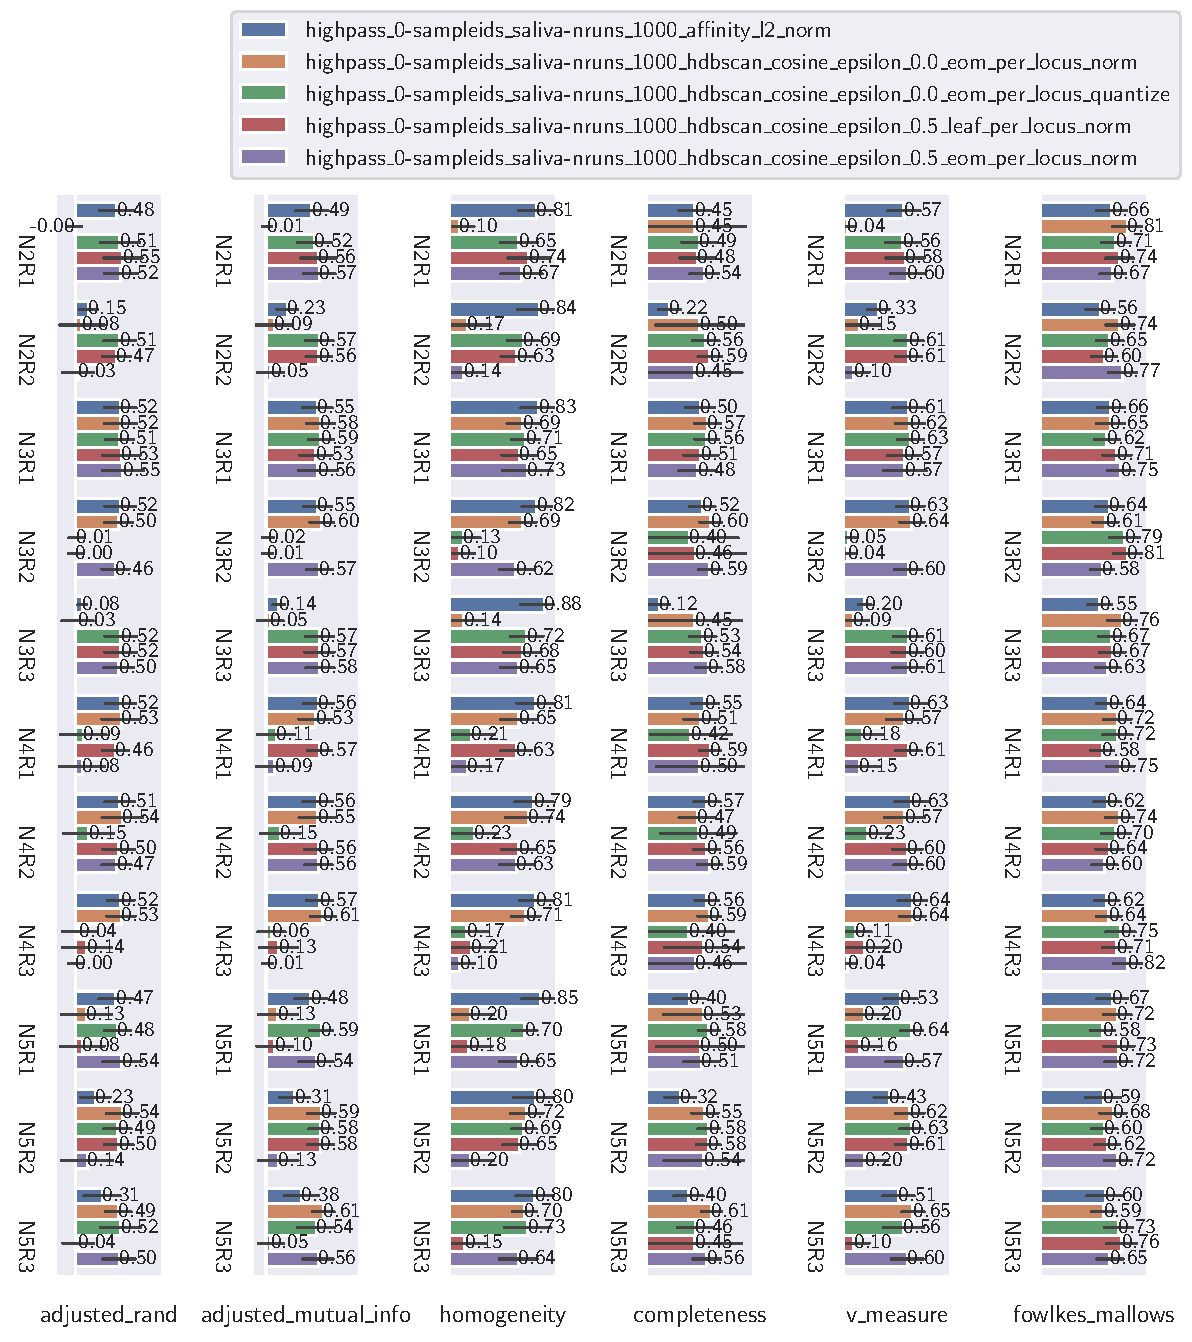
\includegraphics[width=\textwidth]{./figures/clust_comparison/highpass_0-sampleids_saliva-nruns_1000_top_5_clusterers_including_ensembles_by_metrics.pdf}
\caption{Top 5 clusterers, including ensembles, clustering performance metrics using 1000 trials sampled from EPGs from only saliva samples without high-pass filtering}
\label{fig:highpass_0-sampleids_saliva-nruns_1000_top_5_clusterers_including_ensembles_by_metrics}
\end{figure}

\begin{table}[H]
\centering
\maxsizebox{\textwidth}{0.65\textwidth}{
\begin{tabular}{lrr}
\toprule
{} &  mean &   std \\
clusterer                                      &       &       \\
\midrule
meanshift\_per\_locus\_norm                       & 1.13\% & 2.13\% \\
meanshift\_per\_locus\_quantize                   & 1.03\% & 2.05\% \\
birch\_l2\_norm                                  & 0.21\% & 0.27\% \\
hdbscan\_cosine\_epsilon\_1.0\_eom\_per\_locus\_norm  & 0.18\% & 0.25\% \\
hdbscan\_cosine\_epsilon\_1.0\_leaf\_per\_locus\_norm & 0.18\% & 0.25\% \\
mclust\_l2\_norm                                 & 0.18\% & 0.28\% \\
hdbscan\_cosine\_epsilon\_0.0\_eom\_per\_locus\_norm  & 0.17\% & 0.24\% \\
hdbscan\_cosine\_epsilon\_0.5\_eom\_per\_locus\_norm  & 0.17\% & 0.24\% \\
hdbscan\_cosine\_epsilon\_0.5\_leaf\_per\_locus\_norm & 0.17\% & 0.24\% \\
optics\_l2\_norm                                 & 0.16\% & 0.22\% \\
\bottomrule
\end{tabular}


}
\caption{Top 10 clusterers by arithmetic mean of percentages of perfect clustering, using admixtures sampled from only saliva EPG data without highpass filter}
\label{table:top_10_clusterers_by_binomial_confidence_highpass_0-sampleids_saliva-nruns_1000}
\end{table}

\begin{table}[H]
\centering
\maxsizebox{\textwidth}{0.65\textwidth}{
\begin{tabular}{llrrrrrrrrrr}
\toprule
     & {} & \multicolumn{5}{l}{homogeneity} & \multicolumn{5}{l}{completeness} \\
     & clusterer &           1 &      2 &      3 &      4 &      5 &            1 &      2 &     3 &      4 &      5 \\
\midrule
N2R1 & ci\_upp &       0.38\% &  3.19\% &  0.38\% &  0.38\% &  0.38\% &       42.67\% & 14.16\% & 0.73\% & 39.43\% &  0.38\% \\
     & success &       0.00\% &  2.10\% &  0.00\% &  0.00\% &  0.00\% &       39.60\% & 12.00\% & 0.20\% & 36.40\% &  0.00\% \\
     & ci\_low &       0.00\% &  1.38\% &  0.00\% &  0.00\% &  0.00\% &       36.61\% & 10.13\% & 0.05\% & 33.48\% &  0.00\% \\
N2R2 & ci\_upp &       0.38\% &  0.38\% &  0.38\% &  0.38\% & 10.83\% &       56.18\% & 32.61\% & 1.30\% &  0.38\% &  0.88\% \\
     & success &       0.00\% &  0.00\% &  0.00\% &  0.00\% &  8.90\% &       53.10\% & 29.70\% & 0.60\% &  0.00\% &  0.30\% \\
     & ci\_low &       0.00\% &  0.00\% &  0.00\% &  0.00\% &  7.29\% &       50.00\% & 26.95\% & 0.28\% &  0.00\% &  0.10\% \\
N3R1 & ci\_upp &       0.38\% & 22.07\% &  0.38\% &  0.56\% &  0.38\% &       35.16\% & 10.28\% & 0.38\% & 45.99\% & 40.85\% \\
     & success &       0.00\% & 19.50\% &  0.00\% &  0.10\% &  0.00\% &       32.20\% &  8.40\% & 0.00\% & 42.90\% & 37.80\% \\
     & ci\_low &       0.00\% & 17.16\% &  0.00\% &  0.02\% &  0.00\% &       29.38\% &  6.84\% & 0.00\% & 39.87\% & 34.85\% \\
N3R2 & ci\_upp &       0.38\% &  0.38\% &  0.38\% &  1.02\% &  1.02\% &       54.88\% & 52.40\% & 0.38\% &  1.57\% &  1.57\% \\
     & success &       0.00\% &  0.00\% &  0.00\% &  0.40\% &  0.40\% &       51.80\% & 49.30\% & 0.00\% &  0.80\% &  0.80\% \\
     & ci\_low &       0.00\% &  0.00\% &  0.00\% &  0.16\% &  0.16\% &       48.70\% & 46.21\% & 0.00\% &  0.41\% &  0.41\% \\
N3R3 & ci\_upp &       6.98\% &  1.57\% &  1.02\% &  0.38\% &  0.38\% &        8.53\% & 12.66\% & 1.02\% &  0.38\% &  0.38\% \\
     & success &       5.40\% &  0.80\% &  0.40\% &  0.00\% &  0.00\% &        6.80\% & 10.60\% & 0.40\% &  0.00\% &  0.00\% \\
     & ci\_low &       4.16\% &  0.41\% &  0.16\% &  0.00\% &  0.00\% &        5.40\% &  8.84\% & 0.16\% &  0.00\% &  0.00\% \\
N4R1 & ci\_upp &       3.31\% &  0.38\% &  0.88\% &  0.38\% &  0.38\% &       19.24\% & 40.54\% & 0.88\% &  0.38\% &  0.38\% \\
     & success &       2.20\% &  0.00\% &  0.30\% &  0.00\% &  0.00\% &       16.80\% & 37.50\% & 0.30\% &  0.00\% &  0.00\% \\
     & ci\_low &       1.46\% &  0.00\% &  0.10\% &  0.00\% &  0.00\% &       14.61\% & 34.55\% & 0.10\% &  0.00\% &  0.00\% \\
N4R2 & ci\_upp &       1.02\% &  0.38\% &  0.38\% & 10.83\% &  0.56\% &       13.84\% & 43.17\% & 0.38\% &  0.88\% & 45.99\% \\
     & success &       0.40\% &  0.00\% &  0.00\% &  8.90\% &  0.10\% &       11.70\% & 40.10\% & 0.00\% &  0.30\% & 42.90\% \\
     & ci\_low &       0.16\% &  0.00\% &  0.00\% &  7.29\% &  0.02\% &        9.85\% & 37.11\% & 0.00\% &  0.10\% & 39.87\% \\
N4R3 & ci\_upp &       0.38\% &  5.40\% &  0.38\% &  0.38\% &  0.38\% &       43.88\% &  4.71\% & 0.38\% & 40.85\% & 36.18\% \\
     & success &       0.00\% &  4.00\% &  0.00\% &  0.00\% &  0.00\% &       40.80\% &  3.40\% & 0.00\% & 37.80\% & 33.20\% \\
     & ci\_low &       0.00\% &  2.95\% &  0.00\% &  0.00\% &  0.00\% &       37.79\% &  2.44\% & 0.00\% & 34.85\% & 30.35\% \\
N5R1 & ci\_upp &       2.09\% & 10.50\% &  9.30\% &  0.38\% &  0.38\% &        6.08\% &  7.20\% & 0.38\% & 36.18\% & 39.43\% \\
     & success &       1.20\% &  8.60\% &  7.50\% &  0.00\% &  0.00\% &        4.60\% &  5.60\% & 0.00\% & 33.20\% & 36.40\% \\
     & ci\_low &       0.69\% &  7.02\% &  6.03\% &  0.00\% &  0.00\% &        3.47\% &  4.34\% & 0.00\% & 30.35\% & 33.48\% \\
N5R2 & ci\_upp &      19.45\% &  0.38\% &  0.38\% &  0.38\% &  0.38\% &       12.45\% & 54.19\% & 0.56\% &  0.38\% &  0.38\% \\
     & success &      17.00\% &  0.00\% &  0.00\% &  0.00\% &  0.00\% &       10.40\% & 51.10\% & 0.10\% &  0.00\% &  0.00\% \\
     & ci\_low &      14.80\% &  0.00\% &  0.00\% &  0.00\% &  0.00\% &        8.66\% & 48.00\% & 0.02\% &  0.00\% &  0.00\% \\
N5R3 & ci\_upp &      44.08\% & 47.60\% & 12.77\% &  0.38\% &  0.38\% &       15.12\% & 14.37\% & 0.73\% &  0.38\% &  0.38\% \\
     & success &      41.00\% & 44.50\% & 10.70\% &  0.00\% &  0.00\% &       12.90\% & 12.20\% & 0.20\% &  0.00\% &  0.00\% \\
     & ci\_low &      37.99\% & 41.45\% &  8.93\% &  0.00\% &  0.00\% &       10.96\% & 10.31\% & 0.05\% &  0.00\% &  0.00\% \\
\bottomrule
\end{tabular}


}
\caption{Top 5 clusterers, including ensembles, clustering percentages of trials where no error occurs using 1000 trials sampled from EPGs from only saliva samples without high-pass filtering}
\label{table:highpass_0-sampleids_saliva-nruns_1000_top_5_clusterers_including_ensembles_by_binomial_confidence}
\end{table}

\subsection{Saliva Samples Only, with High-Pass Filtering}

\begin{table}[H]
\centering
\maxsizebox{\textwidth}{0.65\textwidth}{
\begin{tabular}{lrr}
\toprule
{} &      mean &       std \\
clusterer                   &           &           \\
\midrule
mclust\_l2\_norm              &  0.896614 &  0.186136 \\
mclust\_l1\_norm              &  0.872849 &  0.196642 \\
birch\_per\_locus\_quantize    &  0.869840 &  0.170125 \\
birch\_per\_locus\_norm        &  0.869058 &  0.173117 \\
cluster\_ensemble\_mcla       &  0.838775 &  0.235953 \\
birch\_l2\_norm               &  0.835254 &  0.195881 \\
affinity\_per\_locus\_quantize &  0.834774 &  0.260209 \\
cluster\_ensemble\_all        &  0.832766 &  0.247135 \\
affinity\_per\_locus\_norm     &  0.812169 &  0.271186 \\
affinity\_l1\_norm            &  0.805911 &  0.269273 \\
\bottomrule
\end{tabular}


}
\caption{Top 10 clusterers, including ensembles, by arithmetic mean of clustering metric scores, using admixtures sampled from only saliva EPG data with highpass filter}
\label{table:top_10_clusterers_by_metrics_highpass_71-sampleids_saliva-nruns_1000}
\end{table}

\begin{figure}[H]
\centering
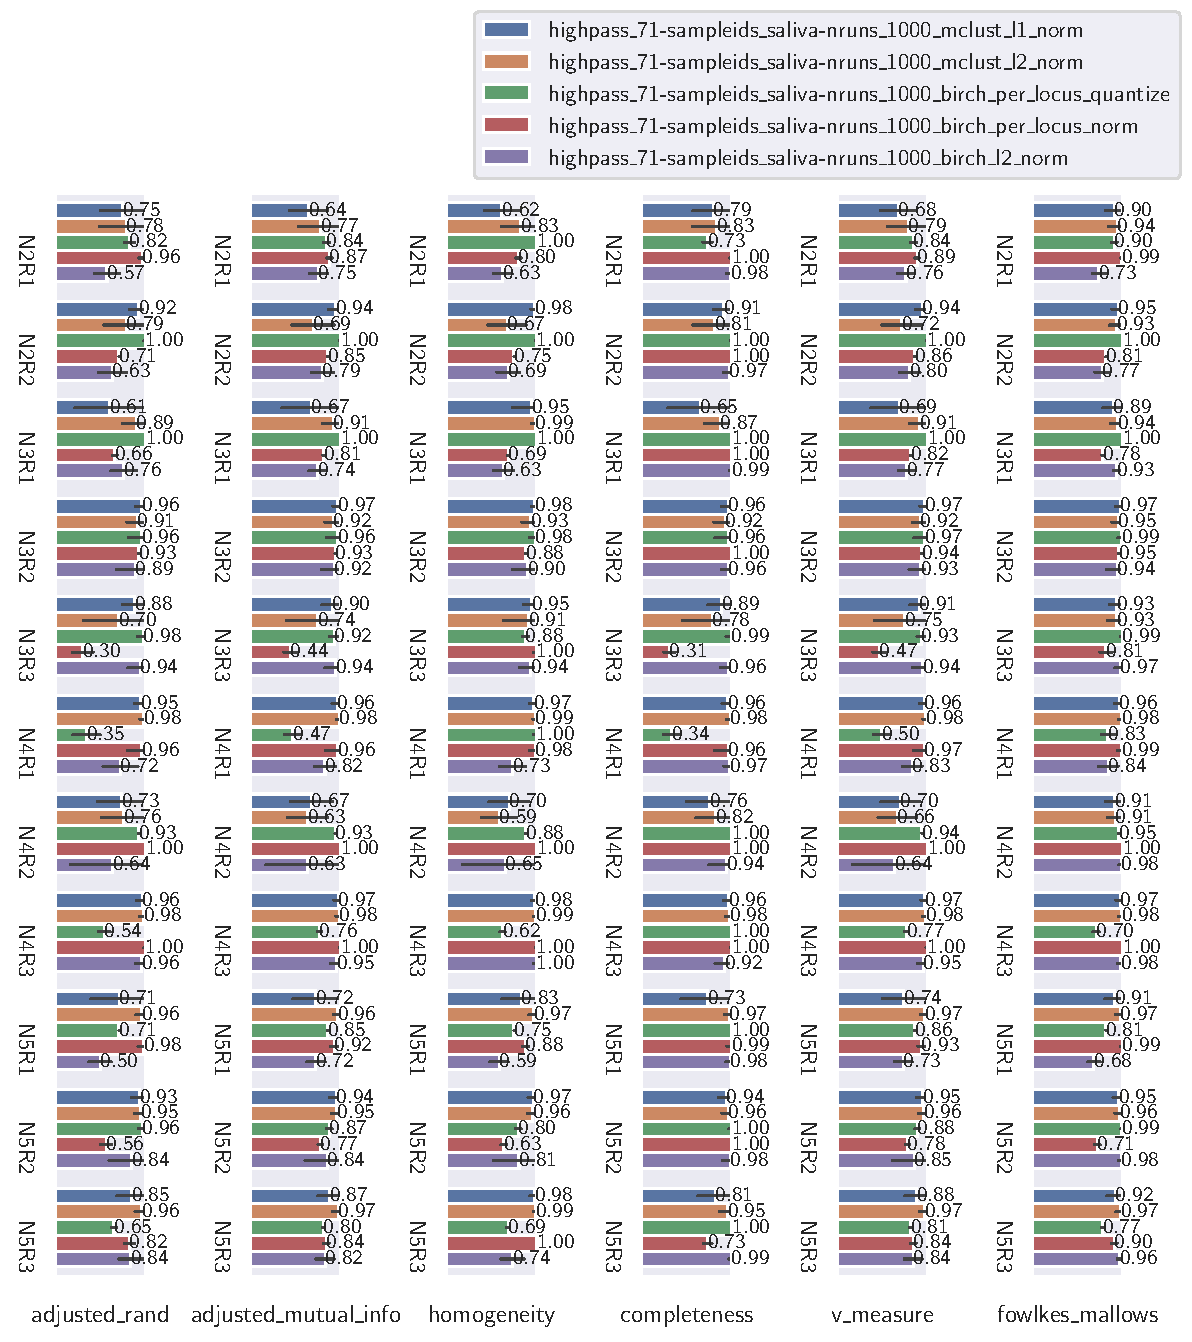
\includegraphics[width=\textwidth]{./figures/clust_comparison/highpass_71-sampleids_saliva-nruns_1000_top_5_clusterers_including_ensembles_by_metrics.pdf}
\caption{Top 5 clusterers, including ensembles, clustering performance metrics using 1000 trials sampled from EPGs from only saliva samples with high-pass filtering}
\label{fig:highpass_71-sampleids_saliva-nruns_1000_top_5_clusterers_including_ensembles_by_metrics}
\end{figure}

\begin{table}[H]
\centering
\maxsizebox{\textwidth}{0.65\textwidth}{
\begin{tabular}{lrr}
\toprule
{} &   mean &    std \\
clusterer                                          &        &        \\
\midrule
hdbscan\_euclidean\_epsilon\_0.0\_eom\_per\_locus\_norm   & 59.08\% & 46.44\% \\
hdbscan\_euclidean\_epsilon\_1.0\_eom\_per\_locus\_norm   & 59.08\% & 46.44\% \\
hdbscan\_euclidean\_epsilon\_0.5\_eom\_per\_locus\_norm   & 59.08\% & 46.44\% \\
hdbscan\_cosine\_epsilon\_0.0\_eom\_per\_locus\_norm      & 58.84\% & 46.75\% \\
hdbscan\_euclidean\_epsilon\_0.0\_eom\_per\_locus\_qua... & 57.91\% & 45.62\% \\
hdbscan\_euclidean\_epsilon\_0.5\_eom\_l2\_norm          & 52.04\% & 41.79\% \\
hdbscan\_euclidean\_epsilon\_0.0\_eom\_l2\_norm          & 52.04\% & 41.79\% \\
hdbscan\_cosine\_epsilon\_0.0\_eom                     & 50.17\% & 40.41\% \\
affinity\_per\_locus\_quantize                        & 49.54\% & 38.19\% \\
hdbscan\_euclidean\_epsilon\_0.5\_leaf\_l2\_norm         & 49.15\% & 39.64\% \\
\bottomrule
\end{tabular}


}
\caption{Top 10 clusterers by arithmetic mean of percentages of perfect clustering, using admixtures sampled from only saliva EPG data with highpass filter}
\label{table:top_10_clusterers_by_binomial_confidence_highpass_71-sampleids_saliva-nruns_1000}
\end{table}

\begin{table}[H]
\centering
\maxsizebox{\textwidth}{0.65\textwidth}{
\begin{tabular}{llrrrrrrrrrr}
\toprule
     & {} & \multicolumn{5}{l}{homogeneity} & \multicolumn{5}{l}{completeness} \\
     & clusterer &           1 &       2 &       3 &       4 &       5 &            1 &      2 &      3 &      4 &      5 \\
\midrule
N2R1 & ci\_upp &     100.00\% & 100.00\% &  98.70\% &  98.70\% &   0.38\% &       99.72\% & 99.09\% & 98.86\% & 99.53\% & 66.04\% \\
     & success &     100.00\% & 100.00\% &  98.00\% &  98.00\% &   0.00\% &       99.40\% & 98.50\% & 98.20\% & 99.10\% & 63.10\% \\
     & ci\_low &      99.62\% &  99.62\% &  96.93\% &  96.93\% &   0.00\% &       98.70\% & 97.54\% & 97.17\% & 98.30\% & 60.06\% \\
N2R2 & ci\_upp &       0.38\% & 100.00\% &   0.38\% &  98.86\% & 100.00\% &       52.10\% & 99.38\% & 38.41\% & 99.95\% & 97.30\% \\
     & success &       0.00\% & 100.00\% &   0.00\% &  98.20\% & 100.00\% &       49.00\% & 98.90\% & 35.40\% & 99.80\% & 96.30\% \\
     & ci\_low &       0.00\% &  99.62\% &   0.00\% &  97.17\% &  99.62\% &       45.91\% & 98.04\% & 32.50\% & 99.27\% & 94.94\% \\
N3R1 & ci\_upp &     100.00\% &  99.01\% &   0.38\% & 100.00\% &  99.98\% &       99.09\% & 99.53\% & 47.60\% & 99.53\% & 97.47\% \\
     & success &     100.00\% &  98.40\% &   0.00\% & 100.00\% &  99.90\% &       98.50\% & 99.10\% & 44.50\% & 99.10\% & 96.50\% \\
     & ci\_low &      99.62\% &  97.42\% &   0.00\% &  99.62\% &  99.44\% &       97.54\% & 98.30\% & 41.45\% & 98.30\% & 95.17\% \\
N3R2 & ci\_upp &      99.01\% &   0.38\% & 100.00\% & 100.00\% &   0.38\% &       99.53\% & 52.89\% & 99.38\% & 99.95\% & 53.99\% \\
     & success &      98.40\% &   0.00\% & 100.00\% & 100.00\% &   0.00\% &       99.10\% & 49.80\% & 98.90\% & 99.80\% & 50.90\% \\
     & ci\_low &      97.42\% &   0.00\% &  99.62\% &  99.62\% &   0.00\% &       98.30\% & 46.71\% & 98.04\% & 99.27\% & 47.80\% \\
N3R3 & ci\_upp &       0.38\% &   0.38\% &  64.56\% &  58.06\% & 100.00\% &       38.41\% & 38.41\% & 80.17\% & 82.27\% & 98.30\% \\
     & success &       0.00\% &   0.00\% &  61.60\% &  55.00\% & 100.00\% &       35.40\% & 35.40\% & 77.70\% & 79.90\% & 97.50\% \\
     & ci\_low &       0.00\% &   0.00\% &  58.55\% &  51.90\% &  99.62\% &       32.50\% & 32.50\% & 75.02\% & 77.30\% & 96.34\% \\
N4R1 & ci\_upp &     100.00\% &   0.38\% &   0.38\% &   0.38\% & 100.00\% &       98.78\% & 47.60\% & 52.89\% & 36.18\% & 99.53\% \\
     & success &     100.00\% &   0.00\% &   0.00\% &   0.00\% & 100.00\% &       98.10\% & 44.50\% & 49.80\% & 33.20\% & 99.10\% \\
     & ci\_low &      99.62\% &   0.00\% &   0.00\% &   0.00\% &  99.62\% &       97.05\% & 41.45\% & 46.71\% & 30.35\% & 98.30\% \\
N4R2 & ci\_upp &      98.70\% & 100.00\% & 100.00\% &   0.38\% &  62.01\% &       98.86\% & 98.78\% & 98.78\% & 50.90\% & 79.98\% \\
     & success &      98.00\% & 100.00\% & 100.00\% &   0.00\% &  59.00\% &       98.20\% & 98.10\% & 98.10\% & 47.80\% & 77.50\% \\
     & ci\_low &      96.93\% &  99.62\% &  99.62\% &   0.00\% &  55.92\% &       97.17\% & 97.05\% & 97.05\% & 44.72\% & 74.81\% \\
N4R3 & ci\_upp &     100.00\% &  98.70\% & 100.00\% & 100.00\% &  98.78\% &       99.38\% & 98.86\% & 99.72\% & 99.84\% & 98.38\% \\
     & success &     100.00\% &  98.00\% & 100.00\% & 100.00\% &  98.10\% &       98.90\% & 98.20\% & 99.40\% & 99.60\% & 97.60\% \\
     & ci\_low &      99.62\% &  96.93\% &  99.62\% &  99.62\% &  97.05\% &       98.04\% & 97.17\% & 98.70\% & 98.98\% & 96.45\% \\
N5R1 & ci\_upp &      64.56\% & 100.00\% & 100.00\% &   0.38\% &  98.70\% &       80.17\% & 99.72\% & 99.09\% & 43.88\% & 96.19\% \\
     & success &      61.60\% & 100.00\% & 100.00\% &   0.00\% &  98.00\% &       77.70\% & 99.40\% & 98.50\% & 40.80\% & 95.00\% \\
     & ci\_low &      58.55\% &  99.62\% &  99.62\% &   0.00\% &  96.93\% &       75.02\% & 98.70\% & 97.54\% & 37.79\% & 93.47\% \\
N5R2 & ci\_upp &       0.38\% &   0.38\% &  99.01\% &   0.38\% &   0.38\% &       47.60\% & 52.10\% & 99.53\% & 50.70\% & 44.98\% \\
     & success &       0.00\% &   0.00\% &  98.40\% &   0.00\% &   0.00\% &       44.50\% & 49.00\% & 99.10\% & 47.60\% & 41.90\% \\
     & ci\_low &       0.00\% &   0.00\% &  97.42\% &   0.00\% &   0.00\% &       41.45\% & 45.91\% & 98.30\% & 44.52\% & 38.88\% \\
N5R3 & ci\_upp &       0.38\% &  64.56\% &   0.38\% & 100.00\% &   0.56\% &       52.89\% & 80.17\% & 52.10\% & 99.38\% & 64.66\% \\
     & success &       0.00\% &  61.60\% &   0.00\% & 100.00\% &   0.10\% &       49.80\% & 77.70\% & 49.00\% & 98.90\% & 61.70\% \\
     & ci\_low &       0.00\% &  58.55\% &   0.00\% &  99.62\% &   0.02\% &       46.71\% & 75.02\% & 45.91\% & 98.04\% & 58.65\% \\
\bottomrule
\end{tabular}


}
\caption{Top 5 clusterers, including ensembles, clustering percentages of trials where no error occurs using 1000 trials sampled from EPGs from only saliva samples with high-pass filtering}
\label{table:highpass_71-sampleids_saliva-nruns_1000_top_5_clusterers_including_ensembles_by_binomial_confidence}
\end{table}

\subsection{Blood Samples Only, without High-Pass Filtering}

\begin{table}[H]
\centering
\maxsizebox{\textwidth}{0.65\textwidth}{
\begin{tabular}{lrr}
\toprule
{} &      mean &       std \\
clusterer                                          &           &           \\
\midrule
mclust\_l1\_norm                                     &  0.793301 &  0.184282 \\
mclust\_l2\_norm                                     &  0.787556 &  0.192270 \\
cluster\_ensemble\_mcla                              &  0.783506 &  0.181843 \\
cluster\_ensemble\_all                               &  0.782045 &  0.184286 \\
affinity\_per\_locus\_quantize                        &  0.746803 &  0.229369 \\
birch\_per\_locus\_norm                               &  0.745169 &  0.188504 \\
birch\_per\_locus\_quantize                           &  0.745103 &  0.188918 \\
hdbscan\_euclidean\_epsilon\_0.0\_eom\_per\_locus\_qua... &  0.731431 &  0.270606 \\
hdbscan\_euclidean\_epsilon\_0.0\_eom\_per\_locus\_norm   &  0.726765 &  0.274433 \\
hdbscan\_euclidean\_epsilon\_1.0\_eom\_per\_locus\_norm   &  0.726765 &  0.274433 \\
\bottomrule
\end{tabular}


}
\caption{Top 10 clusterers, including ensembles, by arithmetic mean of clustering metric scores, using admixtures sampled from only blood EPG data without highpass filter}
\label{table:top_10_clusterers_by_metrics_highpass_0-sampleids_blood-nruns_1000}
\end{table}

\begin{figure}[H]
\centering
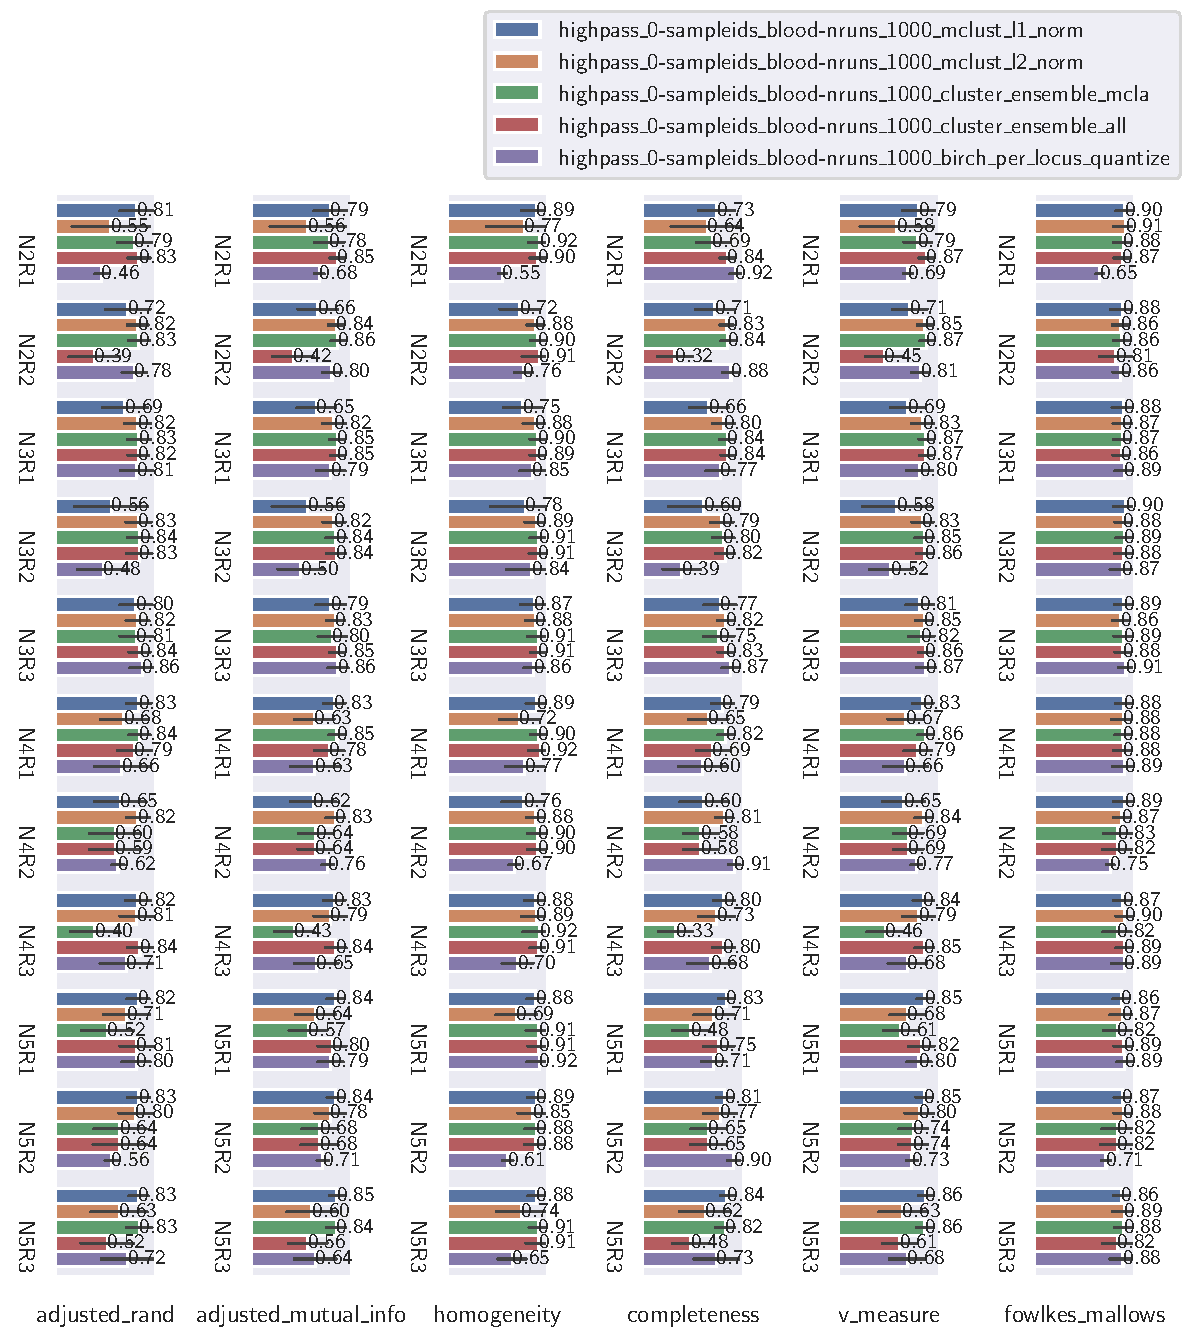
\includegraphics[width=\textwidth]{./figures/clust_comparison/highpass_0-sampleids_blood-nruns_1000_top_5_clusterers_including_ensembles_by_metrics.pdf}
\caption{Top 5 clusterers, including ensembles, clustering performance metrics using 1000 trials sampled from EPGs from only blood samples without high-pass filtering}
\label{fig:highpass_0-sampleids_blood-nruns_1000_top_5_clusterers_including_ensembles_by_metrics}
\end{figure}

\begin{table}[H]
\centering
\maxsizebox{\textwidth}{0.65\textwidth}{
\begin{tabular}{lrr}
\toprule
{} &  mean &    std \\
clusterer                                          &       &        \\
\midrule
mclust\_l2\_norm                                     & 9.10\% & 10.15\% \\
mclust\_l1\_norm                                     & 8.92\% &  9.30\% \\
hdbscan\_euclidean\_epsilon\_0.0\_eom\_per\_locus\_qua... & 4.98\% &  7.95\% \\
hdbscan\_euclidean\_epsilon\_0.5\_eom\_per\_locus\_norm   & 4.90\% &  7.89\% \\
hdbscan\_euclidean\_epsilon\_0.0\_eom\_per\_locus\_norm   & 4.90\% &  7.89\% \\
hdbscan\_euclidean\_epsilon\_1.0\_eom\_per\_locus\_norm   & 4.90\% &  7.89\% \\
affinity\_per\_locus\_quantize                        & 3.75\% &  4.93\% \\
affinity\_per\_locus\_norm                            & 3.61\% &  5.16\% \\
birch\_per\_locus\_norm                               & 3.39\% &  5.53\% \\
birch\_per\_locus\_quantize                           & 3.35\% &  5.47\% \\
\bottomrule
\end{tabular}


}
\caption{Top 10 clusterers by arithmetic mean of percentages of perfect clustering, using admixtures sampled from only blood EPG data without highpass filter}
\label{table:top_10_clusterers_by_binomial_confidence_highpass_0-sampleids_blood-nruns_1000}
\end{table}

\begin{table}[H]
\centering
\maxsizebox{\textwidth}{0.65\textwidth}{
\begin{tabular}{llrrrrrrrrrr}
\toprule
     & {} & \multicolumn{5}{l}{homogeneity} & \multicolumn{5}{l}{completeness} \\
     & clusterer &           1 &      2 &      3 &      4 &      5 &            1 &      2 &      3 &      4 &      5 \\
\midrule
N2R1 & ci\_upp &      69.84\% & 40.95\% &  0.38\% &  4.37\% & 48.00\% &       50.30\% & 21.44\% & 23.22\% &  1.83\% & 29.01\% \\
     & success &      67.00\% & 37.90\% &  0.00\% &  3.10\% & 44.90\% &       47.20\% & 18.90\% & 20.60\% &  1.00\% & 26.20\% \\
     & ci\_low &      64.03\% & 34.94\% &  0.00\% &  2.19\% & 41.84\% &       44.12\% & 16.59\% & 18.21\% &  0.54\% & 23.57\% \\
N2R2 & ci\_upp &       1.02\% & 16.61\% &  2.21\% & 33.53\% & 15.01\% &        0.73\% & 16.08\% & 26.95\% & 23.94\% &  7.65\% \\
     & success &       0.40\% & 14.30\% &  1.30\% & 30.60\% & 12.80\% &        0.20\% & 13.80\% & 24.20\% & 21.30\% &  6.00\% \\
     & ci\_low &       0.16\% & 12.27\% &  0.76\% & 27.82\% & 10.87\% &        0.05\% & 11.80\% & 21.65\% & 18.87\% &  4.69\% \\
N3R1 & ci\_upp &       8.64\% & 23.53\% & 12.12\% &  1.44\% & 12.23\% &        4.83\% & 13.41\% &  7.54\% &  0.56\% &  7.54\% \\
     & success &       6.90\% & 20.90\% & 10.10\% &  0.70\% & 10.20\% &        3.50\% & 11.30\% &  5.90\% &  0.10\% &  5.90\% \\
     & ci\_low &       5.49\% & 18.49\% &  8.38\% &  0.34\% &  8.47\% &        2.53\% &  9.48\% &  4.60\% &  0.02\% &  4.60\% \\
N3R2 & ci\_upp &      10.61\% & 67.01\% & 48.30\% & 22.49\% & 33.53\% &        6.64\% & 44.38\% & 29.42\% & 18.61\% & 23.94\% \\
     & success &       8.70\% & 64.10\% & 45.20\% & 19.90\% & 30.60\% &        5.10\% & 41.30\% & 26.60\% & 16.20\% & 21.30\% \\
     & ci\_low &       7.11\% & 61.08\% & 42.14\% & 17.54\% & 27.82\% &        3.90\% & 38.29\% & 23.95\% & 14.05\% & 18.87\% \\
N3R3 & ci\_upp &       2.95\% & 29.84\% &  5.29\% &  0.56\% &  0.56\% &        1.83\% & 20.08\% &  2.34\% & 19.24\% & 19.24\% \\
     & success &       1.90\% & 27.00\% &  3.90\% &  0.10\% &  0.10\% &        1.00\% & 17.60\% &  1.40\% & 16.80\% & 16.80\% \\
     & ci\_low &       1.22\% & 24.34\% &  2.87\% &  0.02\% &  0.02\% &        0.54\% & 15.36\% &  0.84\% & 14.61\% & 14.61\% \\
N4R1 & ci\_upp &      20.19\% & 11.26\% & 14.91\% & 12.23\% &  0.38\% &       12.45\% &  6.19\% &  7.98\% &  7.54\% & 18.82\% \\
     & success &      17.70\% &  9.30\% & 12.70\% & 10.20\% &  0.00\% &       10.40\% &  4.70\% &  6.30\% &  5.90\% & 16.40\% \\
     & ci\_low &      15.46\% &  7.65\% & 10.78\% &  8.47\% &  0.00\% &        8.66\% &  3.55\% &  4.95\% &  4.60\% & 14.23\% \\
N4R2 & ci\_upp &       3.78\% & 35.67\% &  4.25\% &  0.38\% &  4.37\% &        2.46\% & 19.56\% &  1.96\% & 18.82\% &  1.83\% \\
     & success &       2.60\% & 32.70\% &  3.00\% &  0.00\% &  3.10\% &        1.50\% & 17.10\% &  1.10\% & 16.40\% &  1.00\% \\
     & ci\_low &       1.78\% & 29.86\% &  2.11\% &  0.00\% &  2.19\% &        0.91\% & 14.89\% &  0.62\% & 14.23\% &  0.54\% \\
N4R3 & ci\_upp &      41.35\% &  9.19\% & 33.01\% & 48.00\% &  5.74\% &       22.49\% &  4.83\% & 31.17\% & 29.01\% &  2.58\% \\
     & success &      38.30\% &  7.40\% & 30.10\% & 44.90\% &  4.30\% &       19.90\% &  3.50\% & 28.30\% & 26.20\% &  1.60\% \\
     & ci\_low &      35.34\% &  5.94\% & 27.34\% & 41.84\% &  3.21\% &       17.54\% &  2.53\% & 25.60\% & 23.57\% &  0.99\% \\
N5R1 & ci\_upp &      13.95\% &  3.31\% &  1.70\% &  0.38\% &  0.38\% &       16.82\% &  1.83\% &  0.38\% & 18.19\% & 18.19\% \\
     & success &      11.80\% &  2.20\% &  0.90\% &  0.00\% &  0.00\% &       14.50\% &  1.00\% &  0.00\% & 15.80\% & 15.80\% \\
     & ci\_low &       9.95\% &  1.46\% &  0.47\% &  0.00\% &  0.00\% &       12.45\% &  0.54\% &  0.00\% & 13.67\% & 13.67\% \\
N5R2 & ci\_upp &      29.12\% &  3.66\% &  0.38\% &  5.74\% & 22.49\% &       20.92\% &  1.83\% & 22.28\% &  2.58\% & 18.61\% \\
     & success &      26.30\% &  2.50\% &  0.00\% &  4.30\% & 19.90\% &       18.40\% &  1.00\% & 19.70\% &  1.60\% & 16.20\% \\
     & ci\_low &      23.67\% &  1.70\% &  0.00\% &  3.21\% & 17.54\% &       16.12\% &  0.54\% & 17.35\% &  0.99\% & 14.05\% \\
N5R3 & ci\_upp &      35.57\% &  1.30\% & 22.70\% & 15.01\% &  1.44\% &       22.49\% &  0.73\% & 18.19\% &  7.65\% &  0.56\% \\
     & success &      32.60\% &  0.60\% & 20.10\% & 12.80\% &  0.70\% &       19.90\% &  0.20\% & 15.80\% &  6.00\% &  0.10\% \\
     & ci\_low &      29.77\% &  0.28\% & 17.73\% & 10.87\% &  0.34\% &       17.54\% &  0.05\% & 13.67\% &  4.69\% &  0.02\% \\
\bottomrule
\end{tabular}


}
\caption{Top 5 clusterers, including ensembles, clustering percentages of trials where no error occurs using 1000 trials sampled from EPGs from only blood samples without high-pass filtering}
\label{table:highpass_0-sampleids_blood-nruns_1000_top_5_clusterers_including_ensembles_by_binomial_confidence}
\end{table}

\subsection{Blood Samples Only, with High-Pass Filtering}

\begin{table}[H]
\centering
\maxsizebox{\textwidth}{0.65\textwidth}{
\begin{tabular}{lrr}
\toprule
{} &      mean &       std \\
clusterer                   &           &           \\
\midrule
mclust\_l1\_norm              &  0.960895 &  0.098183 \\
mclust\_l2\_norm              &  0.953501 &  0.107068 \\
cluster\_ensemble\_mcla       &  0.906558 &  0.168099 \\
cluster\_ensemble\_all        &  0.900609 &  0.183406 \\
birch\_per\_locus\_quantize    &  0.849550 &  0.173975 \\
affinity\_per\_locus\_quantize &  0.844791 &  0.250112 \\
birch\_per\_locus\_norm        &  0.842968 &  0.184070 \\
affinity\_per\_locus\_norm     &  0.792776 &  0.294350 \\
affinity\_l1\_norm            &  0.791961 &  0.290986 \\
affinity\_l2\_norm            &  0.787894 &  0.297917 \\
\bottomrule
\end{tabular}


}
\caption{Top 10 clusterers, including ensembles, by arithmetic mean of clustering metric scores, using admixtures sampled from only blood EPG data with highpass filter}
\label{table:top_10_clusterers_by_metrics_highpass_71-sampleids_blood-nruns_1000}
\end{table}

\begin{figure}[H]
\centering
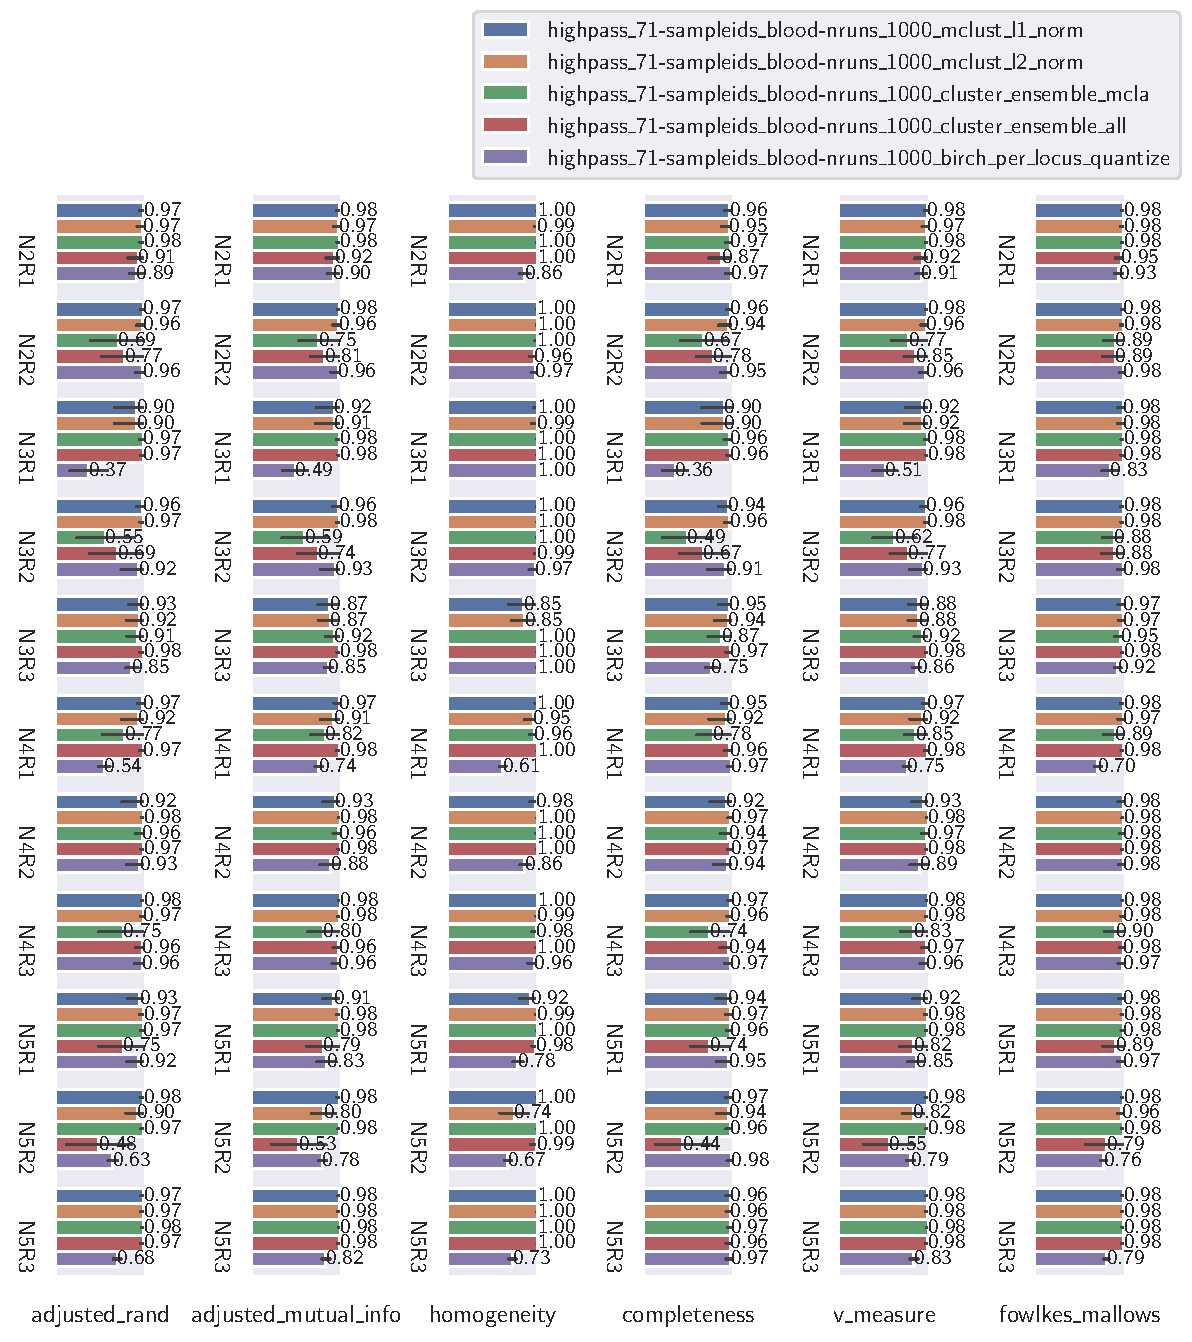
\includegraphics[width=\textwidth]{./figures/clust_comparison/highpass_71-sampleids_blood-nruns_1000_top_5_clusterers_including_ensembles_by_metrics.pdf}
\caption{Top 5 clusterers, including ensembles, clustering performance metrics using 1000 trials sampled from EPGs from only blood samples with high-pass filtering}
\label{fig:highpass_71-sampleids_blood-nruns_1000_top_5_clusterers_including_ensembles_by_metrics}
\end{figure}

\begin{table}[H]
\centering
\maxsizebox{\textwidth}{0.65\textwidth}{
\begin{tabular}{lrr}
\toprule
{} &   mean &    std \\
clusterer                                        &        &        \\
\midrule
mclust\_l1\_norm                                   & 64.13\% & 12.62\% \\
mclust\_l2\_norm                                   & 59.02\% & 18.32\% \\
cluster\_ensemble\_mcla                            & 42.46\% & 22.34\% \\
cluster\_ensemble\_all                             & 42.43\% & 22.43\% \\
affinity\_per\_locus\_quantize                      & 39.18\% & 29.74\% \\
affinity\_per\_locus\_norm                          & 39.05\% & 30.77\% \\
affinity\_l1\_norm                                 & 38.79\% & 30.49\% \\
affinity\_l2\_norm                                 & 38.67\% & 30.44\% \\
hdbscan\_euclidean\_epsilon\_0.0\_eom\_per\_locus\_norm & 36.66\% & 29.52\% \\
hdbscan\_euclidean\_epsilon\_0.5\_eom\_per\_locus\_norm & 36.66\% & 29.52\% \\
\bottomrule
\end{tabular}


}
\caption{Top 10 clusterers by arithmetic mean of percentages of perfect clustering, using admixtures sampled from only blood EPG data with highpass filter}
\label{table:top_10_clusterers_by_binomial_confidence_highpass_71-sampleids_blood-nruns_1000}
\end{table}

\begin{table}[H]
\centering
\maxsizebox{\textwidth}{0.65\textwidth}{
\begin{tabular}{llrrrrrrrrrr}
\toprule
     & {} & \multicolumn{5}{l}{homogeneity} & \multicolumn{5}{l}{completeness} \\
     & clusterer &           1 &      2 &      3 &      4 &      5 &            1 &      2 &      3 &      4 &      5 \\
\midrule
N2R1 & ci\_upp &      98.62\% & 94.69\% & 97.72\% & 99.95\% & 95.93\% &       70.33\% & 78.74\% & 68.97\% & 54.69\% & 68.38\% \\
     & success &      97.90\% & 93.30\% & 96.80\% & 99.80\% & 94.70\% &       67.50\% & 76.20\% & 66.10\% & 51.60\% & 65.50\% \\
     & ci\_low &      96.81\% & 91.58\% & 95.52\% & 99.27\% & 93.13\% &       64.53\% & 73.46\% & 63.11\% & 48.50\% & 62.50\% \\
N2R2 & ci\_upp &      92.17\% & 99.24\% & 98.30\% & 63.19\% & 99.66\% &       55.58\% & 78.45\% & 21.76\% & 17.03\% & 74.50\% \\
     & success &      90.50\% & 98.70\% & 97.50\% & 60.20\% & 99.30\% &       52.50\% & 75.90\% & 19.20\% & 14.70\% & 71.80\% \\
     & ci\_low &      88.52\% & 97.79\% & 96.34\% & 57.13\% & 98.56\% &       49.40\% & 73.15\% & 16.88\% & 12.64\% & 68.93\% \\
N3R1 & ci\_upp &      99.90\% & 99.66\% & 98.70\% & 91.80\% & 97.39\% &       86.61\% & 86.80\% & 69.36\% & 53.49\% & 57.37\% \\
     & success &      99.70\% & 99.30\% & 98.00\% & 90.10\% & 96.40\% &       84.50\% & 84.70\% & 66.50\% & 50.40\% & 54.30\% \\
     & ci\_low &      99.12\% & 98.56\% & 96.93\% & 88.09\% & 95.06\% &       82.13\% & 82.34\% & 63.52\% & 47.31\% & 51.20\% \\
N3R2 & ci\_upp &      99.16\% & 98.62\% & 99.95\% & 97.39\% & 97.39\% &       78.35\% & 70.62\% & 15.33\% & 21.76\% & 51.60\% \\
     & success &      98.60\% & 97.90\% & 99.80\% & 96.40\% & 96.40\% &       75.80\% & 67.80\% & 13.10\% & 19.20\% & 48.50\% \\
     & ci\_low &      97.66\% & 96.81\% & 99.27\% & 95.06\% & 95.06\% &       73.05\% & 64.84\% & 11.15\% & 16.88\% & 45.41\% \\
N3R3 & ci\_upp &      54.49\% & 48.10\% & 99.95\% & 97.81\% & 98.54\% &       86.61\% & 87.83\% & 54.39\% & 69.16\% & 68.77\% \\
     & success &      51.40\% & 45.00\% & 99.80\% & 96.90\% & 97.80\% &       84.50\% & 85.80\% & 51.30\% & 66.30\% & 65.90\% \\
     & ci\_low &      48.30\% & 41.94\% & 99.27\% & 95.63\% & 96.69\% &       82.13\% & 83.50\% & 48.20\% & 63.31\% & 62.91\% \\
N4R1 & ci\_upp &      96.45\% & 77.68\% & 63.48\% & 98.70\% & 91.07\% &       78.45\% & 86.42\% & 17.03\% & 69.36\% &  7.54\% \\
     & success &      95.30\% & 75.10\% & 60.50\% & 98.00\% & 89.30\% &       75.90\% & 84.30\% & 14.70\% & 66.50\% &  5.90\% \\
     & ci\_low &      93.81\% & 72.33\% & 57.44\% & 96.93\% & 87.23\% &       73.15\% & 81.91\% & 12.64\% & 63.52\% &  4.60\% \\
N4R2 & ci\_upp &      89.13\% & 95.05\% & 97.64\% & 94.24\% & 95.13\% &       86.42\% & 53.39\% & 72.37\% & 51.70\% & 74.98\% \\
     & success &      87.20\% & 93.70\% & 96.70\% & 92.80\% & 93.80\% &       84.30\% & 50.30\% & 69.60\% & 48.60\% & 72.30\% \\
     & ci\_low &      84.99\% & 92.02\% & 95.40\% & 91.03\% & 92.13\% &       81.91\% & 47.21\% & 66.68\% & 45.51\% & 69.44\% \\
N4R3 & ci\_upp &      96.88\% & 87.73\% & 83.50\% & 97.64\% & 92.44\% &       53.29\% & 55.48\% & 18.09\% & 72.47\% & 52.00\% \\
     & success &      95.80\% & 85.70\% & 81.20\% & 96.70\% & 90.80\% &       50.20\% & 52.40\% & 15.70\% & 69.70\% & 48.90\% \\
     & ci\_low &      94.37\% & 83.39\% & 78.66\% & 95.40\% & 88.85\% &       47.11\% & 49.30\% & 13.58\% & 66.78\% & 45.81\% \\
N5R1 & ci\_upp &      71.89\% & 92.35\% & 91.89\% & 82.84\% & 83.31\% &       87.64\% & 71.60\% & 53.29\% & 18.09\% & 14.59\% \\
     & success &      69.10\% & 90.70\% & 90.20\% & 80.50\% & 81.00\% &       85.60\% & 68.80\% & 50.20\% & 15.70\% & 12.40\% \\
     & ci\_low &      66.17\% & 88.74\% & 88.20\% & 77.93\% & 78.45\% &       83.29\% & 65.86\% & 47.11\% & 13.58\% & 10.50\% \\
N5R2 & ci\_upp &      95.66\% & 25.71\% & 97.47\% & 96.88\% & 96.36\% &       71.89\% & 86.80\% & 57.96\% & 14.80\% &  5.51\% \\
     & success &      94.40\% & 23.00\% & 96.50\% & 95.80\% & 95.20\% &       69.10\% & 84.70\% & 54.90\% & 12.60\% &  4.10\% \\
     & ci\_low &      92.80\% & 20.50\% & 95.17\% & 94.37\% & 93.69\% &       66.17\% & 82.34\% & 51.80\% & 10.69\% &  3.04\% \\
N5R3 & ci\_upp &      97.30\% & 96.19\% & 97.22\% & 97.47\% & 86.89\% &       59.05\% & 59.05\% & 52.10\% & 57.86\% &  9.19\% \\
     & success &      96.30\% & 95.00\% & 96.20\% & 96.50\% & 84.80\% &       56.00\% & 56.00\% & 49.00\% & 54.80\% &  7.40\% \\
     & ci\_low &      94.94\% & 93.47\% & 94.83\% & 95.17\% & 82.44\% &       52.91\% & 52.91\% & 45.91\% & 51.70\% &  5.94\% \\
\bottomrule
\end{tabular}


}
\caption{Top 5 clusterers, including ensembles, clustering percentages of trials where no error occurs using 1000 trials sampled from EPGs from only blood samples with high-pass filtering}
\label{table:highpass_71-sampleids_blood-nruns_1000_top_5_clusterers_including_ensembles_by_binomial_confidence}
\end{table}

\subsection{All Samples, without High-Pass Filtering}

\begin{table}[H]
\centering
\maxsizebox{\textwidth}{0.65\textwidth}{
\begin{tabular}{lrr}
\toprule
{} &      mean &       std \\
clusterer                                          &           &           \\
\midrule
birch\_per\_locus\_quantize                           &  0.641797 &  0.211116 \\
birch\_per\_locus\_norm                               &  0.641290 &  0.211306 \\
cluster\_ensemble\_mcla                              &  0.639000 &  0.209602 \\
cluster\_ensemble\_all                               &  0.637556 &  0.212475 \\
mclust\_l1\_norm                                     &  0.632317 &  0.234902 \\
mclust\_l2\_norm                                     &  0.628675 &  0.240790 \\
affinity\_per\_locus\_quantize                        &  0.626572 &  0.227781 \\
affinity\_l2\_norm                                   &  0.616125 &  0.234093 \\
hdbscan\_euclidean\_epsilon\_0.0\_eom\_per\_locus\_qua... &  0.606724 &  0.259711 \\
hdbscan\_euclidean\_epsilon\_0.5\_eom\_per\_locus\_norm   &  0.606178 &  0.262164 \\
\bottomrule
\end{tabular}


}
\caption{Top 10 clusterers, including ensembles, by arithmetic mean of clustering metric scores, using admixtures sampled from all EPG data without highpass filter}
\label{table:top_10_clusterers_by_metrics_highpass_0-sampleids_all-nruns_1000}
\end{table}

\begin{figure}[H]
\centering
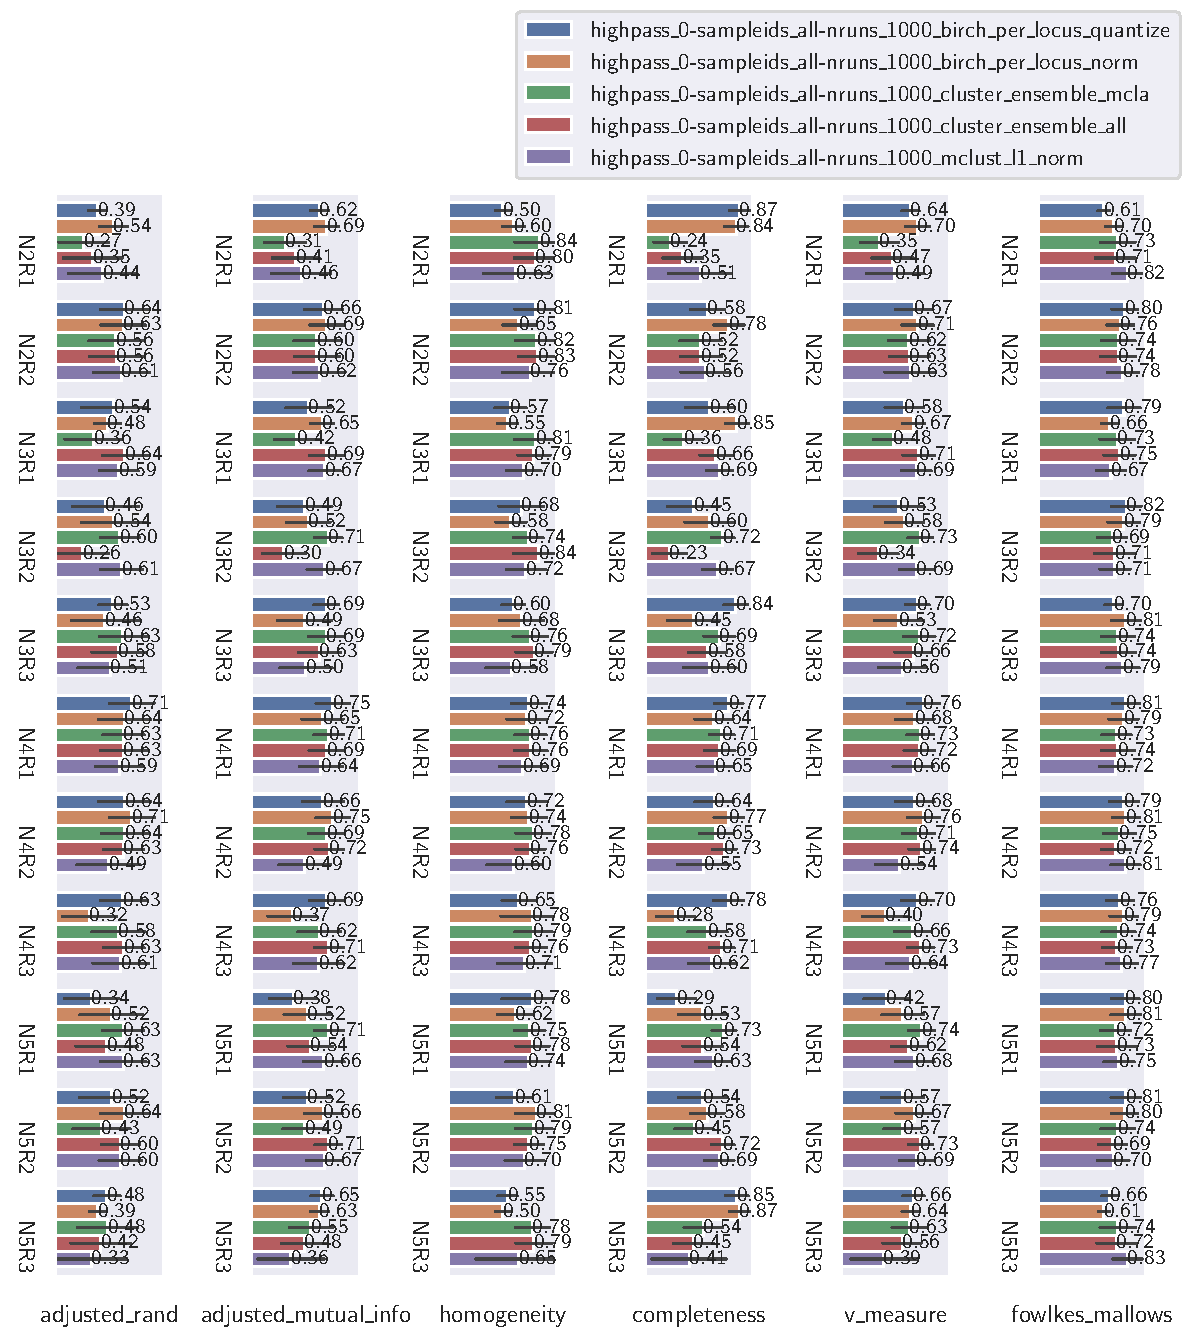
\includegraphics[width=\textwidth]{./figures/clust_comparison/highpass_0-sampleids_all-nruns_1000_top_5_clusterers_including_ensembles_by_metrics.pdf}
\caption{Top 5 clusterers, including ensembles, clustering performance metrics using 1000 trials sampled from all EPGs without high-pass filtering}
\label{fig:highpass_0-sampleids_all-nruns_1000_top_5_clusterers_including_ensembles_by_metrics}
\end{figure}

\begin{table}[H]
\centering
\maxsizebox{\textwidth}{0.65\textwidth}{
\begin{tabular}{lrr}
\toprule
{} &  mean &   std \\
clusterer                                          &       &       \\
\midrule
mclust\_l2\_norm                                     & 3.09\% & 4.12\% \\
mclust\_l1\_norm                                     & 2.97\% & 3.75\% \\
meanshift\_per\_locus\_norm                           & 2.66\% & 2.49\% \\
hdbscan\_euclidean\_epsilon\_1.0\_eom\_per\_locus\_norm   & 2.39\% & 4.63\% \\
hdbscan\_euclidean\_epsilon\_0.0\_eom\_per\_locus\_norm   & 2.39\% & 4.63\% \\
hdbscan\_euclidean\_epsilon\_0.5\_eom\_per\_locus\_norm   & 2.39\% & 4.63\% \\
hdbscan\_euclidean\_epsilon\_0.0\_eom\_per\_locus\_qua... & 2.23\% & 4.47\% \\
meanshift\_per\_locus\_quantize                       & 1.91\% & 1.98\% \\
birch\_per\_locus\_quantize                           & 1.78\% & 2.88\% \\
birch\_per\_locus\_norm                               & 1.73\% & 2.79\% \\
\bottomrule
\end{tabular}


}
\caption{Top 10 clusterers by arithmetic mean of percentages of perfect clustering, using admixtures sampled from all EPG data without highpass filter}
\label{table:top_10_clusterers_by_binomial_confidence_highpass_0-sampleids_all-nruns_1000}
\end{table}

\begin{table}[H]
\centering
\maxsizebox{\textwidth}{0.65\textwidth}{
\begin{tabular}{llrrrrrrrrrr}
\toprule
     & {} & \multicolumn{5}{l}{homogeneity} & \multicolumn{5}{l}{completeness} \\
     & clusterer &           1 &      2 &      3 &      4 &      5 &            1 &      2 &      3 &      4 &      5 \\
\midrule
N2R1 & ci\_upp &       2.46\% & 23.63\% & 21.23\% &  3.66\% &  0.88\% &        1.57\% & 19.66\% &  8.86\% &  4.71\% &  1.44\% \\
     & success &       1.50\% & 21.00\% & 18.70\% &  2.50\% &  0.30\% &        0.80\% & 17.20\% &  7.10\% &  3.40\% &  0.70\% \\
     & ci\_low &       0.91\% & 18.59\% & 16.40\% &  1.70\% &  0.10\% &        0.41\% & 14.99\% &  5.67\% &  2.44\% &  0.34\% \\
N2R2 & ci\_upp &       4.48\% & 27.57\% & 27.16\% &  0.38\% &  6.64\% &        1.57\% &  9.30\% &  7.76\% &  0.38\% &  4.83\% \\
     & success &       3.20\% & 24.80\% & 24.40\% &  0.00\% &  5.10\% &        0.80\% &  7.50\% &  6.10\% &  0.00\% &  3.50\% \\
     & ci\_low &       2.28\% & 22.22\% & 21.84\% &  0.00\% &  3.90\% &        0.41\% &  6.03\% &  4.78\% &  0.00\% &  2.53\% \\
N3R1 & ci\_upp &      22.70\% &  0.38\% &  0.38\% &  1.02\% &  3.66\% &       23.94\% &  0.38\% & 75.18\% &  1.44\% &  4.71\% \\
     & success &      20.10\% &  0.00\% &  0.00\% &  0.40\% &  2.50\% &       21.30\% &  0.00\% & 72.50\% &  0.70\% &  3.40\% \\
     & ci\_low &      17.73\% &  0.00\% &  0.00\% &  0.16\% &  1.70\% &       18.87\% &  0.00\% & 69.65\% &  0.34\% &  2.44\% \\
N3R2 & ci\_upp &       0.73\% &  0.88\% &  0.38\% &  6.64\% &  0.38\% &        0.73\% &  0.73\% & 76.24\% &  4.83\% &  0.38\% \\
     & success &       0.20\% &  0.30\% &  0.00\% &  5.10\% &  0.00\% &        0.20\% &  0.20\% & 73.60\% &  3.50\% &  0.00\% \\
     & ci\_low &       0.05\% &  0.10\% &  0.00\% &  3.90\% &  0.00\% &        0.05\% &  0.05\% & 70.78\% &  2.53\% &  0.00\% \\
N3R3 & ci\_upp &       0.38\% &  5.17\% & 17.45\% & 11.04\% &  0.38\% &        0.38\% & 14.27\% &  9.19\% & 12.77\% & 12.02\% \\
     & success &       0.00\% &  3.80\% & 15.10\% &  9.10\% &  0.00\% &        0.00\% & 12.10\% &  7.40\% & 10.70\% & 10.00\% \\
     & ci\_low &       0.00\% &  2.78\% & 13.01\% &  7.47\% &  0.00\% &        0.00\% & 10.22\% &  5.94\% &  8.93\% &  8.29\% \\
N4R1 & ci\_upp &      53.59\% &  2.58\% & 68.09\% &  0.38\% & 11.04\% &       29.73\% &  1.70\% &  9.52\% & 12.98\% & 12.77\% \\
     & success &      50.50\% &  1.60\% & 65.20\% &  0.00\% &  9.10\% &       26.90\% &  0.90\% &  7.70\% & 10.90\% & 10.70\% \\
     & ci\_low &      47.41\% &  0.99\% & 62.19\% &  0.00\% &  7.47\% &       24.24\% &  0.47\% &  6.20\% &  9.12\% &  8.93\% \\
N4R2 & ci\_upp &       8.75\% &  9.08\% & 33.73\% &  0.38\% &  0.38\% &       14.59\% & 11.04\% &  7.65\% & 12.45\% & 12.45\% \\
     & success &       7.00\% &  7.30\% & 30.80\% &  0.00\% &  0.00\% &       12.40\% &  9.10\% &  6.00\% & 10.40\% & 10.40\% \\
     & ci\_low &       5.58\% &  5.85\% & 28.02\% &  0.00\% &  0.00\% &       10.50\% &  7.47\% &  4.69\% &  8.66\% &  8.66\% \\
N4R3 & ci\_upp &       0.73\% & 14.59\% &  7.31\% & 30.56\% & 30.56\% &        0.88\% &  8.64\% & 13.73\% & 20.19\% & 20.19\% \\
     & success &       0.20\% & 12.40\% &  5.70\% & 27.70\% & 27.70\% &        0.30\% &  6.90\% & 11.60\% & 17.70\% & 17.70\% \\
     & ci\_low &       0.05\% & 10.50\% &  4.43\% & 25.02\% & 25.02\% &        0.10\% &  5.49\% &  9.76\% & 15.46\% & 15.46\% \\
N5R1 & ci\_upp &      14.59\% &  5.06\% & 43.27\% &  0.88\% & 19.56\% &       10.28\% &  1.96\% & 12.12\% &  1.44\% & 13.09\% \\
     & success &      12.40\% &  3.70\% & 40.20\% &  0.30\% & 17.10\% &        8.40\% &  1.10\% & 10.10\% &  0.70\% & 11.00\% \\
     & ci\_low &      10.50\% &  2.70\% & 37.20\% &  0.10\% & 14.89\% &        6.84\% &  0.62\% &  8.38\% &  0.34\% &  9.21\% \\
N5R2 & ci\_upp &      27.36\% &  0.56\% &  0.38\% &  0.38\% &  1.02\% &        9.63\% &  0.73\% & 72.95\% & 12.02\% &  1.44\% \\
     & success &      24.60\% &  0.10\% &  0.00\% &  0.00\% &  0.40\% &        7.80\% &  0.20\% & 70.20\% & 10.00\% &  0.70\% \\
     & ci\_low &      22.03\% &  0.02\% &  0.00\% &  0.00\% &  0.16\% &        6.29\% &  0.05\% & 67.29\% &  8.29\% &  0.34\% \\
N5R3 & ci\_upp &       4.25\% & 52.69\% &  4.48\% & 19.56\% &  0.38\% &       16.08\% & 24.78\% & 22.80\% & 13.09\% & 12.98\% \\
     & success &       3.00\% & 49.60\% &  3.20\% & 17.10\% &  0.00\% &       13.80\% & 22.10\% & 20.20\% & 11.00\% & 10.90\% \\
     & ci\_low &       2.11\% & 46.51\% &  2.28\% & 14.89\% &  0.00\% &       11.80\% & 19.64\% & 17.83\% &  9.21\% &  9.12\% \\
\bottomrule
\end{tabular}


}
\caption{Top 5 clusterers, including ensembles, clustering percentages of trials where no error occurs using 1000 trials sampled from all EPGs without high-pass filtering}
\label{table:highpass_0-sampleids_all-nruns_1000_top_5_clusterers_including_ensembles_by_binomial_confidence}
\end{table}

\subsection{All Samples, with High-Pass Filtering}

\begin{table}[H]
\centering
\maxsizebox{\textwidth}{0.65\textwidth}{
\begin{tabular}{lrr}
\toprule
{} &      mean &       std \\
clusterer                   &           &           \\
\midrule
mclust\_l2\_norm              &  0.937051 &  0.136490 \\
mclust\_l1\_norm              &  0.936063 &  0.136644 \\
cluster\_ensemble\_mcla       &  0.879164 &  0.193338 \\
cluster\_ensemble\_all        &  0.873449 &  0.206286 \\
birch\_per\_locus\_quantize    &  0.854580 &  0.173664 \\
birch\_per\_locus\_norm        &  0.849947 &  0.181758 \\
affinity\_per\_locus\_quantize &  0.844803 &  0.251359 \\
affinity\_per\_locus\_norm     &  0.799051 &  0.288982 \\
affinity\_l1\_norm            &  0.794859 &  0.285157 \\
birch\_l2\_norm               &  0.794308 &  0.221001 \\
\bottomrule
\end{tabular}


}
\caption{Top 10 clusterers, including ensembles, by arithmetic mean of clustering metric scores, using admixtures sampled from all EPG data with highpass filter}
\label{table:top_10_clusterers_by_metrics_highpass_71-sampleids_all-nruns_1000}
\end{table}

\begin{figure}[H]
\centering
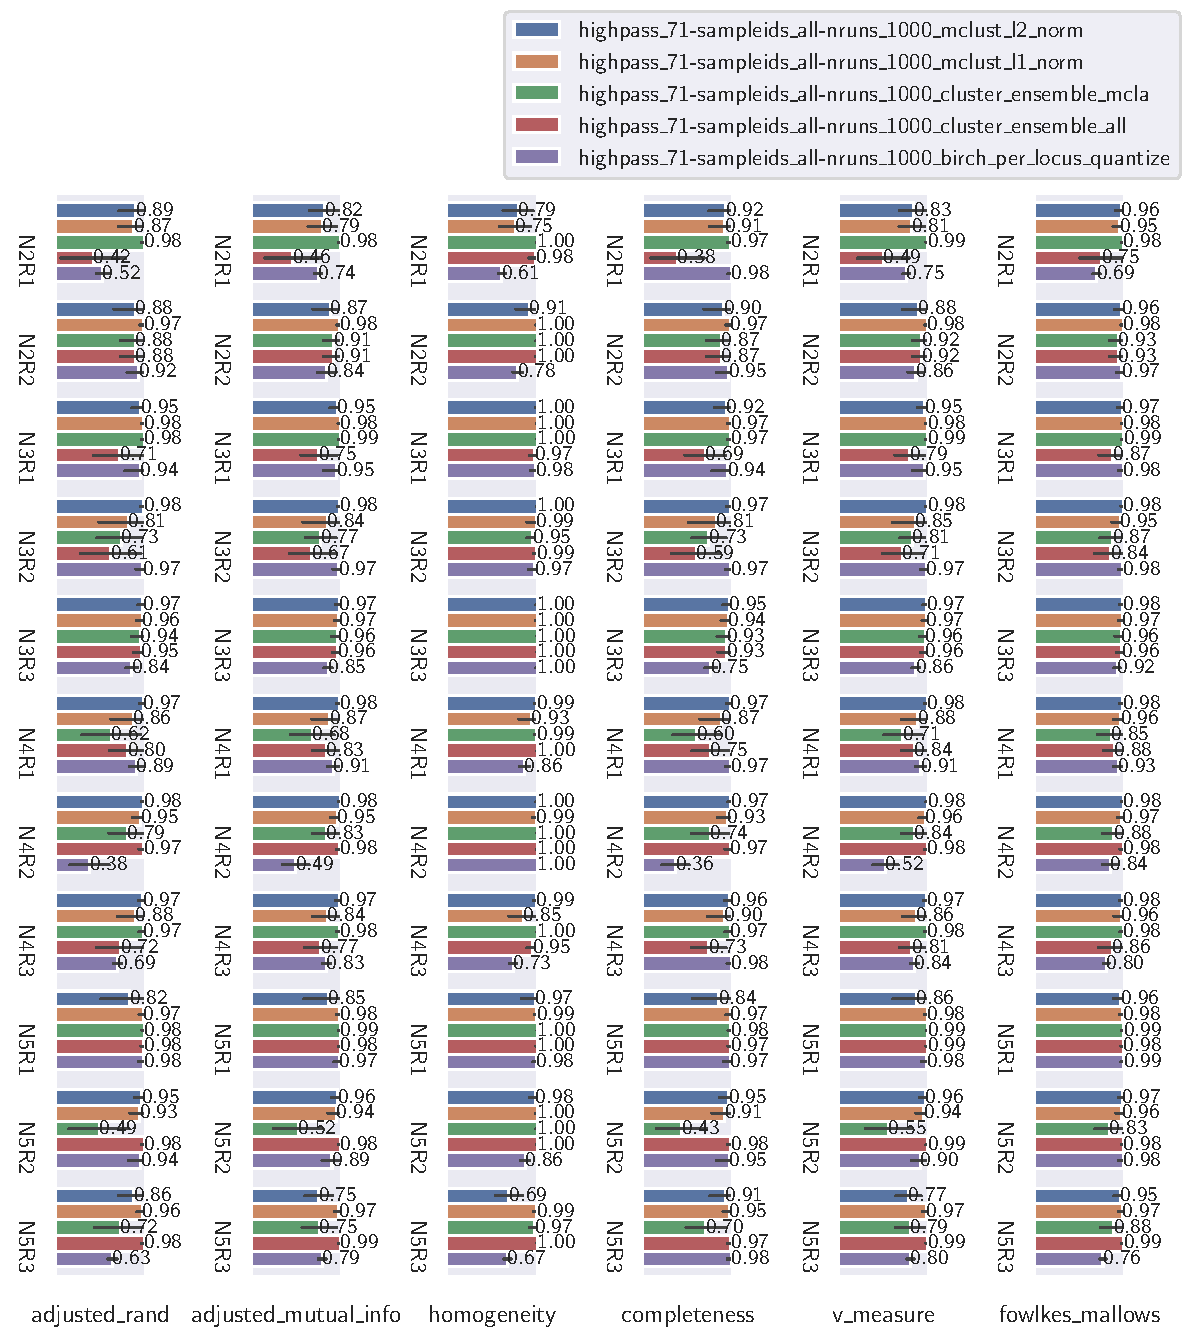
\includegraphics[width=\textwidth]{./figures/clust_comparison/highpass_71-sampleids_all-nruns_1000_top_5_clusterers_including_ensembles_by_metrics.pdf}
\caption{Top 5 clusterers, including ensembles, clustering performance metrics using 1000 trials sampled from all EPGs with high-pass filtering}
\label{fig:highpass_71-sampleids_all-nruns_1000_top_5_clusterers_including_ensembles_by_metrics}
\end{figure}

\begin{table}[H]
\centering
\maxsizebox{\textwidth}{0.65\textwidth}{
\begin{tabular}{lrr}
\toprule
{} &   mean &    std \\
clusterer                                          &        &        \\
\midrule
mclust\_l1\_norm                                     & 55.81\% & 16.52\% \\
mclust\_l2\_norm                                     & 55.11\% & 21.59\% \\
affinity\_per\_locus\_quantize                        & 43.65\% & 33.43\% \\
hdbscan\_cosine\_epsilon\_0.0\_eom\_per\_locus\_norm      & 43.43\% & 34.65\% \\
hdbscan\_euclidean\_epsilon\_0.0\_eom\_per\_locus\_norm   & 43.29\% & 34.62\% \\
hdbscan\_euclidean\_epsilon\_0.5\_eom\_per\_locus\_norm   & 43.29\% & 34.62\% \\
hdbscan\_euclidean\_epsilon\_1.0\_eom\_per\_locus\_norm   & 43.29\% & 34.62\% \\
affinity\_l2\_norm                                   & 42.88\% & 33.43\% \\
affinity\_per\_locus\_norm                            & 42.69\% & 33.26\% \\
hdbscan\_euclidean\_epsilon\_0.0\_eom\_per\_locus\_qua... & 42.66\% & 34.18\% \\
\bottomrule
\end{tabular}


}
\caption{Top 10 clusterers by arithmetic mean of percentages of perfect clustering, using admixtures sampled from all EPG data with highpass filter}
\label{table:top_10_clusterers_by_binomial_confidence_highpass_71-sampleids_all-nruns_1000}
\end{table}

\begin{table}[H]
\centering
\maxsizebox{\textwidth}{0.65\textwidth}{
\begin{tabular}{llrrrrrrrrrr}
\toprule
     & {} & \multicolumn{5}{l}{homogeneity} & \multicolumn{5}{l}{completeness} \\
     & clusterer &           1 &      2 &      3 &      4 &      5 &            1 &      2 &      3 &      4 &      5 \\
\midrule
N2R1 & ci\_upp &      23.94\% & 27.16\% & 97.39\% & 98.62\% &  4.02\% &       77.87\% & 83.97\% & 82.93\% & 86.33\% & 32.09\% \\
     & success &      21.30\% & 24.40\% & 96.40\% & 97.90\% &  2.80\% &       75.30\% & 81.70\% & 80.60\% & 84.20\% & 29.20\% \\
     & ci\_low &      18.87\% & 21.84\% & 95.06\% & 96.81\% &  1.94\% &       72.53\% & 79.18\% & 78.03\% & 81.81\% & 26.47\% \\
N2R2 & ci\_upp &      94.06\% & 64.27\% & 89.31\% & 98.78\% &  0.38\% &       65.06\% & 83.31\% &  9.85\% & 79.02\% & 31.07\% \\
     & success &      92.60\% & 61.30\% & 87.40\% & 98.10\% &  0.00\% &       62.10\% & 81.00\% &  8.00\% & 76.50\% & 28.20\% \\
     & ci\_low &      90.81\% & 58.24\% & 85.20\% & 97.05\% &  0.00\% &       59.05\% & 78.45\% &  6.47\% & 73.77\% & 25.50\% \\
N3R1 & ci\_upp &      90.88\% & 99.01\% & 94.96\% & 98.46\% & 50.60\% &       59.05\% & 76.24\% & 65.64\% & 72.57\% & 70.43\% \\
     & success &      89.10\% & 98.40\% & 93.60\% & 97.70\% & 47.50\% &       56.00\% & 73.60\% & 62.70\% & 69.80\% & 67.60\% \\
     & ci\_low &      87.02\% & 97.42\% & 91.91\% & 96.57\% & 44.42\% &       52.91\% & 70.78\% & 59.66\% & 66.88\% & 64.64\% \\
N3R2 & ci\_upp &      98.94\% & 94.87\% & 94.78\% &  0.38\% & 98.94\% &       75.85\% & 68.09\% &  6.08\% & 32.20\% & 65.55\% \\
     & success &      98.30\% & 93.50\% & 93.40\% &  0.00\% & 98.30\% &       73.20\% & 65.20\% &  4.60\% & 29.30\% & 62.60\% \\
     & ci\_low &      97.29\% & 91.80\% & 91.69\% &  0.00\% & 97.29\% &       70.37\% & 62.19\% &  3.47\% & 26.56\% & 59.56\% \\
N3R3 & ci\_upp &      96.71\% & 97.05\% & 96.27\% &  5.06\% &  0.38\% &       66.33\% & 71.21\% & 72.76\% & 29.01\% & 35.97\% \\
     & success &      95.60\% & 96.00\% & 95.10\% &  3.70\% &  0.00\% &       63.40\% & 68.40\% & 70.00\% & 26.20\% & 33.00\% \\
     & ci\_low &      94.14\% & 94.60\% & 93.58\% &  2.70\% &  0.00\% &       60.37\% & 65.45\% & 67.09\% & 23.57\% & 30.16\% \\
N4R1 & ci\_upp &      74.60\% & 82.74\% & 96.96\% & 98.14\% & 98.62\% &       78.54\% & 62.11\% &  4.25\% & 69.65\% & 72.37\% \\
     & success &      71.90\% & 80.40\% & 95.90\% & 97.30\% & 97.90\% &       76.00\% & 59.10\% &  3.00\% & 66.80\% & 69.60\% \\
     & ci\_low &      69.03\% & 77.83\% & 94.49\% & 96.10\% & 96.81\% &       73.26\% & 56.02\% &  2.11\% & 63.82\% & 66.68\% \\
N4R2 & ci\_upp &      93.53\% & 89.31\% & 98.78\% &  0.38\% &  0.38\% &       74.89\% & 60.63\% & 73.44\% & 26.12\% & 33.22\% \\
     & success &      92.00\% & 87.40\% & 98.10\% &  0.00\% &  0.00\% &       72.20\% & 57.60\% & 70.70\% & 23.40\% & 30.30\% \\
     & ci\_low &      90.15\% & 85.20\% & 97.05\% &  0.00\% &  0.00\% &       69.34\% & 54.51\% & 67.80\% & 20.88\% & 27.53\% \\
N4R3 & ci\_upp &      45.49\% & 87.17\% & 98.70\% &  0.38\% & 97.56\% &       80.65\% & 69.94\% & 66.62\% & 32.40\% & 76.72\% \\
     & success &      42.40\% & 85.10\% & 98.00\% &  0.00\% & 96.60\% &       78.20\% & 67.10\% & 63.70\% & 29.50\% & 74.10\% \\
     & ci\_low &      39.37\% & 82.76\% & 96.93\% &  0.00\% & 95.29\% &       75.54\% & 64.13\% & 60.67\% & 26.76\% & 71.30\% \\
N5R1 & ci\_upp &      85.39\% & 97.89\% & 97.81\% & 97.89\% & 99.16\% &       61.12\% & 79.69\% & 59.15\% & 65.55\% & 78.93\% \\
     & success &      83.20\% & 97.00\% & 96.90\% & 97.00\% & 98.60\% &       58.10\% & 77.20\% & 56.10\% & 62.60\% & 76.40\% \\
     & ci\_low &      80.76\% & 95.75\% & 95.63\% & 95.75\% & 97.66\% &       55.02\% & 74.50\% & 53.01\% & 59.56\% & 73.67\% \\
N5R2 & ci\_upp &      98.62\% & 89.31\% & 99.59\% & 51.90\% & 98.38\% &       71.89\% & 79.41\% & 79.41\% & 71.11\% & 69.65\% \\
     & success &      97.90\% & 87.40\% & 99.20\% & 48.80\% & 97.60\% &       69.10\% & 76.90\% & 76.90\% & 68.30\% & 66.80\% \\
     & ci\_low &      96.81\% & 85.20\% & 98.43\% & 45.71\% & 96.45\% &       66.17\% & 74.19\% & 74.19\% & 65.35\% & 63.82\% \\
N5R3 & ci\_upp &      88.94\% & 11.04\% & 91.98\% & 96.88\% & 99.01\% &       65.84\% & 79.69\% &  8.64\% & 76.43\% & 86.14\% \\
     & success &      87.00\% &  9.10\% & 90.30\% & 95.80\% & 98.40\% &       62.90\% & 77.20\% &  6.90\% & 73.80\% & 84.00\% \\
     & ci\_low &      84.77\% &  7.47\% & 88.31\% & 94.37\% & 97.42\% &       59.86\% & 74.50\% &  5.49\% & 70.99\% & 81.60\% \\
\bottomrule
\end{tabular}


}
\caption{Top 5 clusterers, including ensembles, clustering percentages of trials where no error occurs using 1000 trials sampled from all EPGs with high-pass filtering}
\label{table:highpass_71-sampleids_all-nruns_1000_top_5_clusterers_including_ensembles_by_binomial_confidence}
\end{table}

\subsection{Analysis}

For EPGs from saliva samples only, none of the cluster ensembles perform in the top five, except for the MCLA ensemble, which places fifth in terms of mean metrics scores for high-pass filtered samples.

For EPGs from blood samples only, both without and with high-pass filtering, the MCLA ensembles place within the top five in terms of mean metrics scores although they trail the Mclust clusterers. Therefore, simply using Mclust for EPGs from blood samples appears the best choice.

For EPGs from all samples, the results are less clear. Mclust has the advantage in terms of percentages of perfect clustering both without and with high-pass filtering. In terms of mean metrics scores, Mclust also has the advantage with high-pass filtered data, although other clusterers, including the MCLA ensembles have the advantage with non-filtered data.

It appears that the cluster ensembles methods in general do not do well in terms of percentages of perfect clustering. We think this is a result of percentages of perfect clustering not being the measure by which the cluster ensembles methods compute the best consensus.

%--------------------------------------------------------------------------------------------------------------------------------------------
\section{Summary}

Overall, Mclust demonstrates its strength over a variety of different sample types, especially blood samples. If the EPG data are high-pass filtered, and if only one clusterer can be used, then using Mclust appears to be a sound choice. If more than one clusterer can be used, then supplementing with the MCLA ensembles may be helpful to smooth out weak points of Mclust.

EPGs from saliva samples are the only cases in which Mclust fall short compared to other clustering methods, especially for data without high-pass filtering. There does not appear to be a single best alternative, as different clusterers perform best for different metrics. In real use, a cluster ensemble may be a sound choice for a consensus result, given that it is in general unknowable which clustering method will produce the best result, for the true answer is unknown.
